\chapter{PDZ}
\label{chap:PDZ}

\section{Introduction}

Nous cherchons maintenant, à évaluer la performance de notre modèle CPD sur un ensemble de protéines. Les domaines PDZ (\og Postynaptic density-95 / Discs large / Zonula occludens-1\fg) sont de petits domaines globulaires qui établissent des réseaux d'interactions entre protéines dans la cellule ,voir \citep{Harris01,Hung02,Tonikian08,Gfeller11,Subbaiah11}. Ils forment des interactions spécifiques avec des protéines cibles, généralement en reconnaissant quelques acides aminés à l'extrémité C-terminale. En raison de leur importance biologique, les domaines PDZ et leur interaction avec les protéines cibles ont été largement étudiés et utilisés en conception \texit{in sillico}. Des ligands ont été conçus  pour moduler l'activité de domaines PDZ impliqués dans diverses pathologies \citep{Roberts12,Zheng15}. Des domaines  PDZ et leurs  ligands redessinés ont été utilisés pour élucider les principes du repliement des protéines et de l'évolution \cite{Kong09,Mclaughlin12,Melero14}. Ainsi, ces domaines avec leurs ligands peptidiques fournissent des \og benchmarks\fg pour tester les méthodes informatiques elles-mêmes \cite{Reina02,Schmidt10,Smith10}.

À partir d'une sélection de domaines PDZ, nous optimisons les énergies de référence, paramètres essentiels dans notre modèle, grâce à la méthode du maximum de vraisemblance. La performance du modèle est testée en générant des séquences par Proteus pour chaque protéine de la sélection. Pour cela, nous nous basons sur les résultats précédents, en particulier ceux de la section \ref{BESTprotocol}, pour définir les valeurs des paramètres de l'optimisation du Monte-Carlo. Nous confrontons nos résultats à ceux de la fonction d'énergie de Rosetta , fonction, qui a connu le plus de succès et qui est la plus souvent citée \cite{Baker06b}. Elle comprend un terme de répulsion de Lennard-Jones, un terme Coulomb, un terme de liaison hydrogène,un terme de solvatation Lazaridis-Karplus et des énergies de référence d'état dépliées, mais est plus empirique que la notre. Il y a un grand nombre de paramètres spécifiquement optimisés pour CPD, qui offrent des performances optimales, mais une interprétation physique moins transparente que Proteus qui lui offre la capacité de calculer les énergies libres.
   
La production de nos séquences calculées est effectuée par des simulations Monte-Carlo où toutes les positions de la chaîne polypeptidique sont autorisées à muter librement, excepté celles occupées par une glycine ou une proline qui conservent leur type d'acide aminé. Ces exceptions découlent de la contrainte du backbone fixe, puisque ces deux types d'acides aminés influent sur la structure du squelette. Nous avons alors des milliers de variantes pour chaque domaine étudié. Nos tests comprennent une validation directe et une validation croisée dans laquelle les énergies de référence optimisées sur un sous-ensemble de notre sélection sont utilisées sur un autre sous-ensembles de cette même sélection.

Nous, réalisons également,une série de simulations Monte-Carlo de deux domaines PDZ où le potentiel chimique hydrophobe des types d'acides aminés est progressivement augmenté, polarisant artificiellement la composition de la protéine. Comme le biais hydrophobe augmente, les acides aminés hydrophobes envahissent progressivement la protéine de l'intérieur,formant, à partir d'un certain seuil, un noyau hydrophobe devenu plus grand que naturel.La propension de chaque position du noyau à devenir hydrophobe à un niveau de biais plus ou moins élevé peut être considéré comme un indice d'hydrophobicité déterminé en fonction de la structure qui nous renseigne sur la capacité du cœur à supporter des mutations.

\section{Le modèle d'état déplié}
\subsection{Les énergies de référence}

Nous travaillons avec l'énergie de pliage de la protéine, c'est-à-dire la différence entre
son énergie à l'état replié et son énergie à l'état déplié. Un mouvement élémentaire possible est une \og mutation\fg:
Il s'agit d'une modification du type de chaîne latérale à une position choisie $i$ dans la protéine pliée, en assignant un rotamère particulier à la nouvelle chaîne latérale et de la même modification dans l'état déplié voir les détails au chapitre \ref{chap:methodes}. Pour une séquence $S$ particulière,nous avons introduit l'énergie de l'état dépliée comme:
\begin{equation}
  E^u=\sum_{i\in S}E^r_{t_i}
  \label{eq:unfolded}
\end{equation} 

Avec, $i$ est la position dans la séquence et $t_i$ le type en $i$,la somme se faisant sur tous les résidus de $S$.

Les grandeurs $E_t^r$ sont les  \og énergies de référence\fg (voir section \ref{sec:theo}). Ainsi,Les énergies de référence sont des paramètres essentiels dans le modèle de simulation. 

\subsection{La vraisemblance des énergies de référence}

Notre objectif maintenant est de  déterminer les énergies de référence empiriquement afin que les simulations produisent des fréquences d'acides aminés qui correspondent à un ensemble de valeurs cibles, notamment des valeurs expérimentales. Pour cela, nous choisissons les $E_t^r$ qui maximisent la probabilité de Boltzmann d'un ensemble de séquences expérimentales.
C'est à dire, nous retenons les $E_t^r$ les plus vraisemblables étant donnée l'observation des séquences expérimentales.

Soit $S$ une séquence particulière. Sa probabilité de Boltzmann est:
\begin{equation}
  \label{eq:PDZ_Bolt}
  p(S)=\frac{1}{Z}\exp(-\beta \Delta G_S)
\end{equation}

avec

\begin{equation}
  \label{eq:PDZ_enerpli}
  \Delta G_S=G_S^f - E^u_S
\end{equation}

Où, $\Delta G_S$ est l'énergie libre de repliement de $S$, $G^f_S$ est de l'énergie libre de l'état replié,$\beta =\frac{1}{kT}$ est la température inverse et $Z$ une constante de normalisation (la fonction de partition). En injectant \ref{eq:PDZ_enerpli} dans \ref{eq:PDZ_Bolt}, nous avons alors:
\begin{equation}
kT \ln p(S) = \sum_{i\in S} E^r(t_i) - G^f_S - kT \ln Z = \sum_{t\in aa}n_S(t)E^r_t - G^f_S - kT\ln Z,
\end{equation}
où la somme à droite se fait sur l'ensemble des types d'acides aminés et $n_S(t)$ est le nombre d'acides aminés de type $t$ dans $S$.

Nous considérons maintenant un ensemble $\mathcal{S}$ de $N$ séquences cibles; on appelle $\mathcal{L}$ la probabilité d'observer l'ensemble $\mathcal{S}$ en entier. $\mathcal{L}$ est fonction des paramètres du modèle $E_t^r$.Comme nous voulons le maximum de $\mathcal{L}$ sur les $E_t^r$ , nous nous référons  à  $\mathcal{L}$ comme la vraisemblance des $E_t^r$ \cite{Kleinman06}.

Nous avons:
\begin{equation}
kT \ln \mathcal{L} = \sum_S}\sum_{i \in aa} n_S(t) E^r_t - \sum_S} G^f_S - N kT \ln Z = \sum_{t \in aa} N(t) E^r_t - \sum_S} G^f_S - N kT \ln Z,
\end{equation}
avec $N(t)$ le nombre d'acides aminés de type $t$ dans l'ensemble $\mathcal{S}$.Le facteur de normalisation $Z$ est une somme sur l'ensemble les séquences possibles $\mathcal{R}$:
\begin{equation}
  Z=\sum_{\mathcal{R}} \exp(-\beta \Delta G_{\mathcal{R}}) = \sum_{\mathcal{R}} \exp(-\beta\Delta G^f_{\mathcal{R}}) \Pi_{t\in aa}\exp(\beta n_{\mathcal{R}} (t) E^r_t)
\end{equation} 
Pour maximiser $\mathcal{L}$, nous considérons la dérivé de $Z$ selon chacune des $E_t$:
\begin{equation}
\frac{ \partial Z }{ \partial E^r_t } = 
   \sum_{\mathcal{R}} \beta n_{\mathcal{R}}(t) \exp (-\beta \Delta G^f_{\mathcal{R}}) \Pi_{s \in aa} \exp(\beta n_{\mathcal{R}}(s) E^r_s) 
\end{equation}

Nous avons alors:
\begin{equation}
\frac{kT}{Z} \frac{ \partial Z }{ \partial E^r_t }
   = \frac{ \sum_{\mathcal{R}} n_{\mathcal{R}}(t) \exp(-\beta \Delta G_{\mathcal{R}}) }{ \sum_{\mathcal{R}} \exp(-\beta \Delta G_{\mathcal{R}}) } = \langle n(t) \rangle.
\end{equation}

La quantité à droite est la moyenne de Boltzmann du nombre $n(t)$ des acides aminés de type $t$ sur toutes les séquences possibles. C'est à dire l'espérance mathématique de $n(t)$ selon la probabilité de Boltzman. Mais comme une simulation Monte-Carlo converge vers la distribution de Boltzman, la population moyenne de t que nous obtenons dans nos simulations converge vers la moyenne de Boltzman de $n(t)$.En pratique, nous obtenons cette quantité comme la population moyenne de $t$ dans une simulation Monte-Carlo assez longue. 

Pour que $ln \mathcal{L}$ soit maximal il faut que ses dérivées par rapport à $E_t^r$ soient nulles.

\begin{equation}
\frac{1}{N} \frac{\partial}{\partial E^r_t} \ln {\mathcal L} = \frac{1}{N} \sum_S n_S(t) - \langle n(t) \rangle 
   = \frac{N(t)}{N} - \langle n(t) \rangle
\end{equation}
et donc
\begin{displaymath}
{\mathcal L} \hspace*{2mm} {\rm maximum} \Longrightarrow \frac{N(t)}{N} = \langle n(t) \rangle, 
\hspace*{2mm} \forall t \in {\rm aa}
\label{eq:optimum}
\end{displaymath}

Ainsi, pour maximiser $\mathcal{L}$, nous choisissons les ${E^r_t}$ tels qu'une longue simulation donne les mêmes fréquences d'acides aminés que l'ensemble cible.


\subsection{Recherche du maximum de vraisemblance}


Nous utilisons trois méthodes pour approcher les valeurs ${E^r_t}$.

\begin{itemize}
  \label{enumMeth}
\item La première consiste à avancer dans la direction du gradient de $ln(\mathcal{L})$ en utilisant la règle itérative suivante (voir \cite{Kleinman06}), nous l'appelons méthode linéaire:
\begin{equation} \label {eq:linear}
  E^r_t(n+1) = E^r_t(n) + \alpha \frac{\partial}{\partial E^r_t} \ln(\mathcal{L})=E^r_t(n) + \delta E (n^{exp}_t - \langle n(t)\rangle_n)
\end{equation} 

avec $\alpha$ une constante, $n^{exp}_t = \frac{N(t)}{N}$ la population moyenne d'acide aminé de type t dans l'ensemble ciblé,
$\langle\rangle_n$ indique une moyenne sur une simulation effectuée en utilisant les énergies de références courantes ${E^r_t(n)}$, et $\delta E$ une constante empirique avec la dimension d'une énergie, correspondant à l'amplitude de mise à jour. Cette procédure de mise à jour est répétée jusqu'à convergence. Nous appelons cette méthode, la méthode de mise à jour linéaire.

\item La deuxième méthode est une variante de la première dans laquelle le $\delta E$ n'est pas constant, mais ajusté au cours de la simulation de la façon suivante. On introduit une fonction Proxy $C$ comme outil de mesure rapide de l'état de l'optimisation, de la façon suivante:

\begin{equation} \label {eq:proxy_function}
C =\sum_{t \in aa}(n^{exp}_t - \langle n(t)\rangle_n )^2
\end{equation} 

  Alors, la règle \ref{eq:linear} est utilisée trois fois avec trois valeurs différentes pour le $\delta E$ ceci avec un jeu d'énergie de références identiques. Une interpolation parabolique est effectuée sur les trois valeurs de la fonction $C$ obtenues, le minimum de la parabole est calculé et est utilisé comme $\delta E$ pour le cycle suivant, au terme duquel les énergies sont mises à jour.

\item La troisième méthode, utilisée précédemment \cite{Schmidt08,Simonson13b}, utilise une règle de mise à jour logarithmique:

  \begin{equation} \label{eq:log}
E^r_t (n+1) = E^r_t (n) + kT \, \ln \frac{\langle n(t) \rangle_n}{n_t^{\rm exp}}
\end{equation}

  avec $kT$ l'énergie thermique, fixée empiriquement à $0,5 kcal/mol$. Nous l'appelons la méthode logarithmique. Dans les dernières itérations, certaines valeurs ont tendance à converger lentement,avec des oscillations. Par conséquent, une règle modifiée est ajoutée dans laquelle une énergie au cycle $n$ et l'énergie au cycle  $n-1$ sont moyennée avec un poids respectif de 2/3 et 1/3 afin d'attenuer les vibrations.

\end{itemize}
???? 
Chaque itération, pour le modèle NEA (voir plus bas), a été effectuée avec 500 millions de pas par réplique de REMC, et 100 millions de pas pour le modèle FDB.

\section{Méthodes de calcul}
  
\subsection{Fonction énergétique efficace pour l'état replié}

La matrice énergétique d'une protéine est calculée avec la fonction d'énergie suivante:
\begin{equation}
  E = E_{MM} + E_{GB} + \sum_i \sigma_iA_i
  \label{eq:energy} 
\end{equation}

$E_{MM}$ représentent l'énergie interne de la protéine se compose de six termes, ils sont détaillés en \ref{sub:mecamol}. 
Les autres termes de l'équation \ref{eq:energy}, représente la contribution du solvant. Nous utilisons un modèle de solvant implicite \og Generalized Born + Surface Area\fg ou GBSA (\ref{sub:GB},\ref{eq:SA}):

Ici, $A_i$ est la surface exposée accessible au solvant de l'atome $i$.$\sigma_i$ est un paramètre qui représente la préférence de chaque atome à être exposé ou caché du solvant. Les atomes du soluté sont divisés en quatre groupes avec pour chacun une valeur $\sigma_i$ spécifique en $cal/mol/Å^2$.Nous travaillons avec deux jeux différents pour les $\sigma_i$. Le premier et un jeu déjà utilisé dans différentes études (\cite{Mignon16},\cite{Druart16b}):
non polaire -5,aromatique -40,polaire -80,ionique -100.
et le second proviennent d'une étude plus récente faite dans de notre laboratoire, dans laquelle il a été optimisé
sur un ensemble de protéines PDZ identique à un des notres \ref{Gaillard17}:\label{phiaTG}
non polaire -3,aromatique -1,polaire -9,ionique -9.

Dans les deux cas, on attribue aux atomes d'hydrogène un coefficient de surface de 0. Les surfaces sont calculées par l'algorithme de Lee et Richards \cite{Lee71},  qui est implémenté dans le programme XPLOR \cite{Xplor} et expliqué en \ref{sub:surpairwise}. Les simulations MC utilisent une constante diélectrique pour la protéine $\epsilon_p = 4$ où $8$ (voir la partie Résultats).
Nous utilisons deux variantes du modèle  GB, la méthode NEA pour \og Nativce Environment Approxition\fg et la méthode FDB \og Fluctuating Dielectric Boundary\fg \cite{Villa17}.Elles sont présentées respectivement en \ref{NEA} et \ref{FDB}.

Le champ de force utilisé, Amber ff99SB \cite{Cornell95}, est légèrement modifié pour le CPD, en remplaceant les charges du backbone par un ensemble unifié, obtenu en faisant la moyenne sur l'ensemble des types d'acides aminés et ajuster légèrement pour rendre la partie backbone de chaque acide aminé neutre \cite{Aleksandrov10b}.

\subsection{Les énergies de référence de l'état déplié}

Dans le modèle CPD, l'énergie de l'état dépliée dépend de la composition de la séquence par l'ensemble des énergies de référence $E^r_t$ (équation \ref{eq:unfolded}). Ici, les énergies de référence sont attribuées en fonction des types d'acides aminés t, mais aussi de la position de chaque acide aminé dans la structure repliée à travers son caractère enfoui ou exposé au solvant. Ainsi, pour un type donné, il y a deux valeurs distinctes de $E^r_t$ , une enfuie et une exposée. Cette approche se justifie par les trois éléments suivants.
\begin{itemize}
  
\item Nous supposons que la structure résiduelle est présente dans l'état déplié, de sorte que les acides aminés conservent en partie leur caractère enfui/exposé.
\item Nous supposons que le modèle d'état déplié compense de manière systématique des erreurs dans la fonction d'énergie de l'état plié, de sorte que  la structure pliée contribue indirectement aux énergies de référence.
\item Cette stratégie rend le modèle moins sensible aux variations de la longueur des boucles de surface et au ratio  de résidus de surface sur  enterrés, qui peut varier considérablement selon les homologues (voir plus bas).  
\end{itemize}
Par conséquent, le modèle devrait être transférable à l'intérieur d'une famille de protéines. Distinguer les positions enfouies / exposées double le nombre de paramètres $E^r_t$ à ajuster. Inversement, pour réduire le nombre de paramètres, nous groupons les acides aminés en classes homologues (voir table \ref{tab;AAgroups}). Dans chaque classe c , et pour chaque type de position (enfoui ou exposé), les énergies de référence ont la forme
\begin{displaymath}
E^r_t = E^r_c + \delta E^r_t
\end{displaymath}
$E^r_c$ est un paramètre ajustable,tandis que $\delta E^r_t$ est une constante, calculée comme la différence d'énergie de mécanique moléculaire entre les types d'acides aminés de classe c, supposé en conformation dépliée où chaque acide aminé interagit uniquement avec lui-même et avec le solvant.

    \begin{table}[!htbp]
      \centering

      \begin{tabular}{ccc}

        \toprule
        Groupe & acides aminés & propriétés\\
        \cmidrule{1-3}

        1   & Ala,Cys,Thr & petit\\
        2   & Ser &\\
        \cmidrule{1-3}
        3   & Glu,Asp & chargé négativement\\
        \cmidrule{1-3}
        4   & Gln,Asn & polaire\\
        \cmidrule{1-3}
        5   & Ile,Leu,Val & apolaire\\
        \cmidrule{1-3}
        6   & Met & non polaire\\
        \cmidrule{1-3}
        7   & Hip,Hid,Hie & chargé positivement\\
        8   & Arg \\
        9   & Lys \\
        \cmidrule{1-3}
        10  & Phe,Trp & aromatique\\
        11  & Tyr \\
        \cmidrule{1-3}
        12  & Gly,Pro & non mutable\\
        \bottomrule


      \end{tabular}      
      \caption{Les groupes d'acides aminés utilisés pour l'optimisation des énergies de référence.}
\label{tab:AAgroups}      
    \end{table}


Plus précisément, nous effectuons des simulations MC d'un peptide étendu (le peptide \textit{Syndecan1} ) et calculons les énergies moyennes pour chaque type d'acide aminé à chaque position peptidique (à l'exclusion des positions terminales). Nous prenons les différences entre les types d'acides aminés et les moyennons sur les positions peptidiques.
Pendant, la maximisation de la vraisemblance, $E_c$ est optimisé tandis que $\delta E_t$ est fixe. Pour optimiser les valeurs $E^r_t$, nous utilisons une des trois méthodes de (\ref{enumMeth}) avec comme fréquences cibles les fréquences expérimentales soient des classes d'acides aminés, soient des types d'acides aminés. Le  début d'optimisation se fait sur les classes, puis lorsque la convergence est correctement établie, c'est à dire lorsque la fonction proxy $C$ calculée sur ces classes retourne des valeurs stables et faibles,nous relâchons cette contrainte pour optimiser sur l'ensemble des types d'acide aminés mutables.Typiquement, vingt cycles d'optimisation sont effectués sur les classes, puis encore vingt cycles sur les types.  

\section{Séquences expérimentales et modèles structurels}
\subsection{L'ensemble des protéines PDZ}

Nous sélectionnons huit protéines de la famille PDZ dont les structures cristallographiques sont connues. Aux trois présentes dans l'ensemble étudié au chapitre précédent:  NHREF,Syntenin et DLG2, sont ajoutés les protéines INAD, GRIP, PSD95, Cask et Tiam1.Leur séquence est présenté à la figure \ref{tab:corePDZ}. Cela constitue un ensemble dont le nombre de positions actives, c'est-à-dire les positions qui vont être mutées, est du même ordre pour chaque séquence d'acide aminé.( voir le tableau \ref{tab:protéines_PDZ}).


\begin{table}[!htbp]
  \centering
  \caption{La sélection de domaines protéiques PDZ}
  \begin{tabular}{cccc}
    \toprule
    nom & Code PDB & résidus & nombre de positions actives\\
    \cmidrule{1-4}
    NHREF    & 1G9O  & 9-99    & 76 \\
    INAD     & 1IHJ  & 13-105  & 82 \\
    GRIP     & 1N7E  & 668-761 & 79 \\
    Syntenin & 1R6J  & 193-273 & 72 \\
    DLG2     & 2BYG  & 186-282 & 82 \\
    PSD95    & 3K82  & 305-402 & 80 \\
    Cask     & 1KWA  & 487-568 & 74 \\
    Tiam1    & 4GVD  & 838-930 & 84 \\
    \bottomrule
    
  \end{tabular}      
  \label{tab:protéines_PDZ}      
\end{table}

\subsection{Alignements Blast croisés}
   
Pour caractériser les homologies dans cet ensemble, une série de requêtes BLAST est effectuée sur chaque paire de séquences en utilisant le programme \verb!blastp! avec les options comme indiqué en \ref{SimPfam}. Il apparaît que Syntenin et Tiam1 sont atypiques dans l'ensemble: Il n'y a pas d'homologue avec une E-value inférieure à $10^{-7}$ et plusieurs E-value supérieur à 10. PSD95 est la protéine la plus consensuelle, ayant d'une part une homologie avec toutes les autres à au plus $6$ $10^{-4}$ , et d'autre part ayant $4$ homologues à moins de $2$ $10^{-10}$, pour un pourcentage d'identité compris entre $30$ et $46$.Globalement, il n'y a que peu d'homologies, la plus forte n'étant que de $3$ $10^{-15}$ entre PSD95 et DLG2 pour un pourcentage d'identité de $37$. Les détails sont dans le tableau \ref{tab:Xblast}.



    \begin{table}[!htbp]
%       \raggedleft{}
       \caption{E-value et pourcentage d'identité des alignements Blast native versus native pour nos séquences PDZ.}
       \resizebox{\linewidth}{!}{%

%       \scalebox{0.99}{
      \begin{tabular}{ccccccccc}

        \toprule
        Protein & NHREF        & INAD      & GRIP        & Syntenin        & DLG2       & PSD95       & CASK       & TIAM1 \\
        \cmidrule{1-9}

        NHREF    & 2 $10^{-66}$ (100) & 5 $10^{-10}$ (40) & 2 10^{-3} (25)        & 3 $ 10^{-7}$ (25) & 2 $ 10^{-11}$ (35)     & 1 $ 10^{-12}$ (30) & 5 $ 10^{-5}$ (25) & 9 $ 10^{-7}$(35)\\     
        INAD     & 5 $ 10^{-10}$ (40)  & 3 $ 10^{-68}$ (100)&  2 $ 10^{-7}$ (27)  & [18]         & 2 $ 10^{-8}$ (27)  & 9 $ 10^{-14}$ (46) & 4 $ 10^{-6}$ (35) & [16]    \\
        GRIP     & 2 $10^{-3}$   (25) & 2 $ 10^{-7}$ (27) &  3 $ 10^{-67}$ (100)  & [21]         & 3 $ 10^{-14}$ (36)     & 2 $ 10^{-10}$ (37) & 9 $ 10^{-12}$ (30) & 5 $ 10^{-5}$ (35)\\
        Syntenin & 3 $ 10^{-7}$ (25)  & [18]       &    [21]     & 1 $ 10^{-59}$ (100)        &  [17]              & 1 $ 10^{-6}$ (32) & 7 $10^{-3}$ (32) & [18]    \\
        DLG2     & 2 $ 10^{-11}$ (35) & 2 $ 10^{-8}$ (27) &  3 $ 10^{-14}$ (37) & [17]          & 7 $10^{-71}$ (100)    & 3 $ 10^{-15}$ (37) & 2 $ 10^{-7}$ (28) & 5 $ 10^{-5}$ (41)\\
        PSD95    & 1 $ 10^{-12}$ (30) & 9 $ 10^{-14}$ (46) &  2 $ 10^{-10}$ (36) & 1 $ 10^{-6}$ (32) & 3 $ 10^{-15}$ (37) & 4 $ 10^{-70}$ (100)& 1 $ 10^{-7}$ (27) & 6 $ 10^{-4}$ (33) \\
        Cask     & 5 $ 10^{-5}$ (25) & 4 $ 10^{-6}$ (35) &  9 $ 10^{-12}$ (30)   & 7 $10^{-3}$ (32)     & 2 $ 10^{-7}$ (28)    & 1 $ 10^{-7}$ (27) & 7 $ 10^{-61}$ (100)& 5 $ 10^{-4}$ (33) \\
        Tiam1    & 9 $ 10^{-7}$ (35) &  [16]      &  5 $ 10^{-5}$ (35) & [18]   & 5 $ 10^{-5}$ (41)    & 6 $ 10^{-4}$ (33) & 5 $ 10^{-4}$ (33) & 1 $ 10^{-68}$ (100)\\
        \bottomrule

      \end{tabular}
      }
      {\footnotesize S'il n'y a pas de touche avec une E-value inférieure à $10$,[.] donne le pourcentage d'identité du couple dans l'alignement des 6 séquences sauvages.
}


\label{tab:Xblast}      
    \end{table}

\subsection{Sélection des homologues}


Pour définir les fréquences d'acides aminés cibles nécesaire à la maximiser nos vraisemblances, nous sélectionnons un ensemble de séquences homologues pour chacunes des 6 premières protéines de notre sélection. En effet, nous excluons Cask et Tiam1 pour le calcul des énergies de références. Pour cela, nous effectuons des recherches BLAST avec comme requête la séquence extraite du fichier PDB sur la base de données \og siwwprot + trEmBL \fg d'Uniprot avec la matrice BLOSUM62 et l'option \og Gapped\fg et sans l'option \og filtre\fg.

Nous obtenons un premier ensemble pour chaque cas en nous limitant aux homologues de bonne qualité au regard de la E-value et du pourcentage d'identité, tout en conservant  en même temps une certaine diversité. Cela oblige pour certaines protéines à accepter des E-values plus haute que  $10^{-40}$, notamment INAD et NHREF , respectivement $10^{-32}$ et $10^{-10}$ ,pour avoir un nombre d'homologues suffisant. Ensuite, les redondances les plus flagrantes sont enlevées manuellement. Finalement,les ensembles se composent de 42 à 126 homologues,avec des pourcentages d'identité supérieurs à 66\% excepté pour INAD où il a fallu descendre jusqu'à 38\%. Voir le tableau pour les détails \ref{tab:select_homo}. Les alignements des séquences homologues retenues pour un groupe constitué des 6 premières protéines sont représentés aux figures \ref{{align_homo:NHREF}},\ref{{align_homo:INAD}},\ref{{align_homo:Syntenin}},\ref{{align_homo:GRIP}},\ref{{align_homo:DLG2}} et \ref{{align_homo:PSD95}}.


    \begin{table}[!htbp]
      \centering
      \caption{Sélection des homologues.}
      \begin{tabular}{cccc}

        \toprule
        protéines & \% identité & &\\
        \cmidrule{1-4}
     NHREF  & 62  &    1 $10^{-32}$  &  67-95 \\
     INAD  & 42  &    1 $10^{-10}$  &  38-95 \\
     GRIP  & 48  &    1 $10^{-45}$  &  84-95 \\
     Syntenin  & 85  &    1 $10^{-43}$  &  85-95 \\
     DLG2  & 43  &    1 $10^{-41}$  &  78-95 \\
     PSD95  & 50  &    1 $10^{-46}$  &  81-95 \\
     \cmidrule{1-4}
     Cask  & 126 &    7 $10^{-28}$  &  60-85 \\
     Tiam1 & 50  &    2 $10^{-23}$  &  60-85 \\

        \bottomrule

      \end{tabular}      
      \label{tab:select_homo}      
    \end{table}

\subsection{Alignements des protéines expérimentales et leurs homologues}

%Tandis que les boucles et les chaînes terminales affichent de grands écarts. L'hélice $\alpha_2$ de Tiam1 est tournée légèrement vers l'extérieur par rapport aux trois autres structures (70). La figure 1b illustre la similarité structurale entre les paires de domaines PDZ. Cette similarité est déterminée par l'écart de rms (root mean square) entre  les atomes $C\alpha$ alignés structurellement et par ailleurs les identités des paires de séquences. Les écarts se situent entre $1,0$ et $2,1 \AA$  des identités de séquences entre 17 et 33 \%.La paire Tiam1/Cask on observe une identité de séquence de 33\% et et leur écart structurel de $1,7 \AA$ calculé sur 42 carbones. Les structures de syntenine et GLG2 sont plus similaires, avec une déviation structurale de $1,0 \AA$ calculé sur 60 C $\alpha$ alignés.


Afin d'obtenir une caractérisation structurale de notre sélection de protéines. Nous réalisons en alignement des huit séquences natives, présenté en haut de \ref{tab:corePDZ}. Cet alignement nous sert de base pour la définition d'un alignement structural. Nous pouvons alors définir un cœur hydrophobe de nos protéines \og PDZ \fg , il est représenté au centre de \ref{tab:corePDZ}.Les 14 positions utilisées pour définir le cœur hydrophobe sont bien conservées dans l'alignement \og seed \fg de Pfam, mais pas totalement. L'Arg, Lys et Gln apparaissent à certaines positions, puisque dans de petites protéines comme des domaines PDZ, la longue partie hydrophobe  de ces chaînes latérales peut être enfui dans le noyau tout en permettant à la pointe polaire de la chaîne d'être exposé au solvant. Quelques résidus Asp et Glu apparaissent aussi, dans les endroits où l'alignement des séquences peut ne pas très bien refléter la superposition 3D les chaînes latérales.

    

    \begin{table}[!htbp]
      \centering

      \begin{tabular}{ccccccccc}

        \toprule
        Protein & NHREF        & INAD      & GRIP        & Syntenin        & DLG2       & PSD95       & Cask       & Tiam1 \\
        \cmidrule{1-9}

        NHREF    & 326 &  64 &  15 &  15 &  59 & 112 & 49  &   1  \\     
        INAD    &  64 & 221 &  56 &  -9 &  88 & 107 & 25  &   9  \\
        GRIP    &  15 &  56 & 378 &  24 &  65 &  87 & 90  &  39  \\
        Syntenin    &  15 & -10 &  24 & 311 & -26 &  22 & 42  & -18  \\
        DLG2    &  59 &  88 &  65 & -26 & 325 & 110 & 24  &  22  \\
        PSD95    & 112 & 107 &  87 &  22 & 110 & 325 & 66  &  21  \\
        Cask    &  49 &  25 &  90 &  42 &  23 &  66 & 308 & 37   \\
        Tiam1   &  1  &  10 &  39 & -18 &  22 &  21 & 37  & 371 \\
        \bottomrule


      \end{tabular} 
      \caption{Similarité des séquences expérimentales homologues, pour les 8 protéines PDZ.}
\label{tab:XSIMIL}      
    \end{table}

    \subsection{Similarité des homologues}

Comme nous avons caractérisé les homologies des séquences natives, nous calculons également la similarité des séquences expérimentales homologues pour chaque couple alignés comme en \ref{tab:corePDZ}. Et apparaissent des situations où les similarités sont négatives, c'est le cas chez les homologues à Cask et Syntennin protéines déjà repérées comme éloignées en termes de séquences, avec une valeur de -26 entre DLG2 et Synetnin, -18 entre Tiam1  et Syntenin. Les plus hautes valeurs,excepté les valeurs d'auto-similarité, sont à  112, entre PSD95 et NREF, et 110 pour la similarité entre les protéines PSD95 et DLG2. La similarité moyenne entre deux protéines différentes de notre sélection se situe aux environs de 50. 

    
    \clearpage

   \begin{figure}[t]
     \centering
     \begin{tabular}{c}
       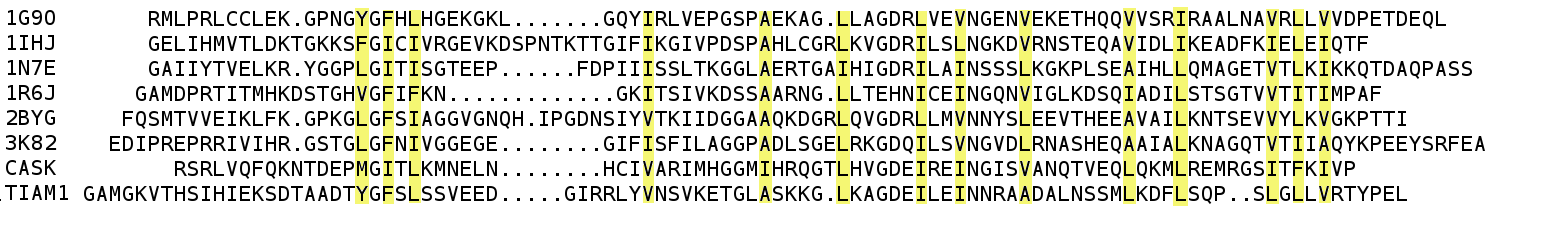
\includegraphics[width=18cm]{images/natives_alignees.png} \\
       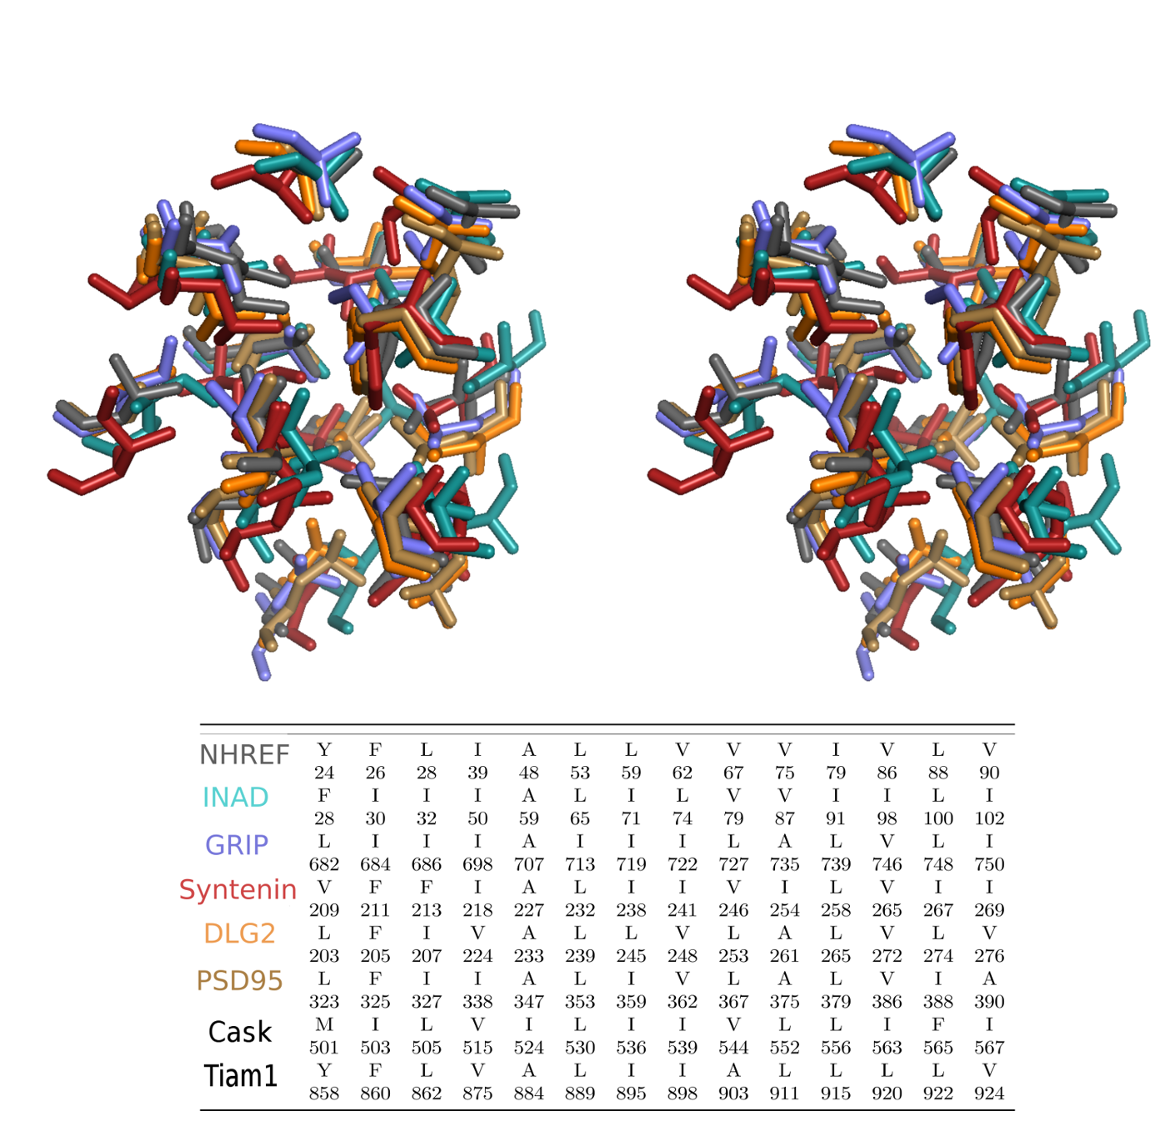
\includegraphics[width=16cm]{images/corePDZ2.png} \\
     \end{tabular}
     \caption{le cœur PDZ sélectionné}
   \end{figure}
    \begin{table}[!htbp]
      \centering

       \label{tab:corePDZ}      
    \end{table}

\subsection{Les fréquences d'acides aminés}

Pour chaque ensemble d'homologues, notons le $\mathcal{H}$, nous calculons des fréquences globales de chaque type d'acide aminé sur toutes les séquences. Les fréquences sont déterminées séparément pour les positions enfouies et pour les positions exposées. Notons les ${f^b_t(\mathcal{H}),f^e_t(\mathcal{H})}$ , où l'indice t représente un type d'acide aminé et les exposants e et b désignent respectivement les ensembles de positions exposées et enfuis. Les ensembles de fréquences moyennes des huit protéines sont divisées selon deux groupes de protéines, d'une part le sous-ensemble $\mathcal{S_1} = \{NHREF,INAD,GRIP,Syntenin,DLG2,PSD95\}$ et d'autre part le groupe $\mathcal{S_2} =\{Cask,Tiam1\}$. Enfin, nous calculons la moyenne des $f^e_t(\mathcal{H})$ et des $f^b_t(\mathcal{H})$ sur $\mathcal{S_1}$ et sur $\mathcal{S_2}$. Cela donne deux jeux de deux ensembles cibles de fréquences d'acides aminés $f^b_t$ et $f^e_t$. Nous faisons la même chose pour chaque classe de type. Cette partition en deux sous-ensembles de protéines va nous permettre d'estimer la transférabilité des énergies de références obtenues à partir d'un sous-ensemble de protéines sur un l'autre.
\label{subsection:freqaa}
        
\clearpage

   \begin{figure}[t]
     \centering
     \begin{tabular}{c}
       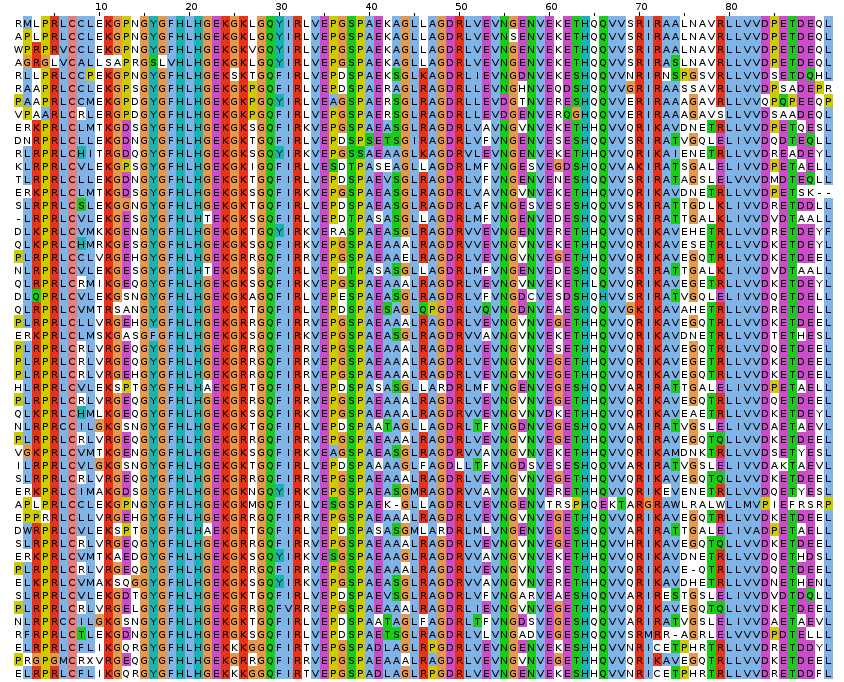
\includegraphics[width=17cm]{homologues/1G9O.png} \\
     \end{tabular}
     \caption{L'alignement de notre sélection de séquences homologues à la protéine NHREF (code PDB:1G9O)}
\label{align_homo:NHREF}
   \end{figure}

   \begin{figure}[t]
     \centering
     \begin{tabular}{c}
       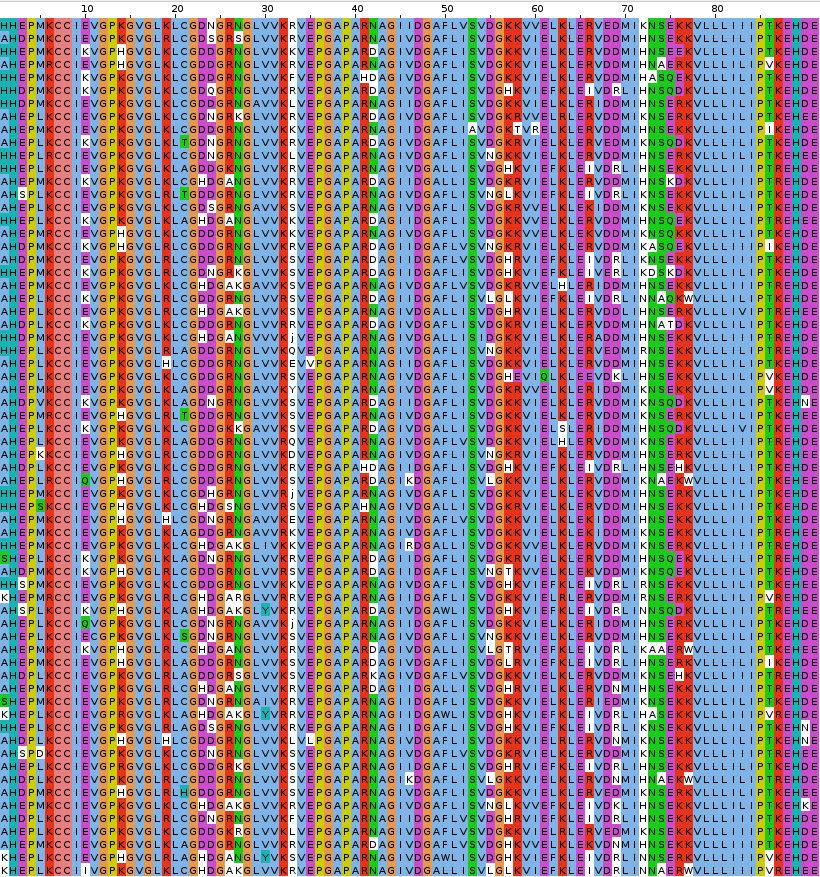
\includegraphics[width=17cm]{proteus/1G9O.png} \\
     \end{tabular}
       \caption{Une sélection de séquences proteus, parmi les 10 000 séquences de meilleure énergie, obtenues avec le backbone de la protéine NHREF (code PDB:1G9O), modèle NEA}
\label{align_proteus:NHREF}
   \end{figure}

\clearpage

   \begin{figure}[t]
     \centering
     \begin{tabular}{c}
       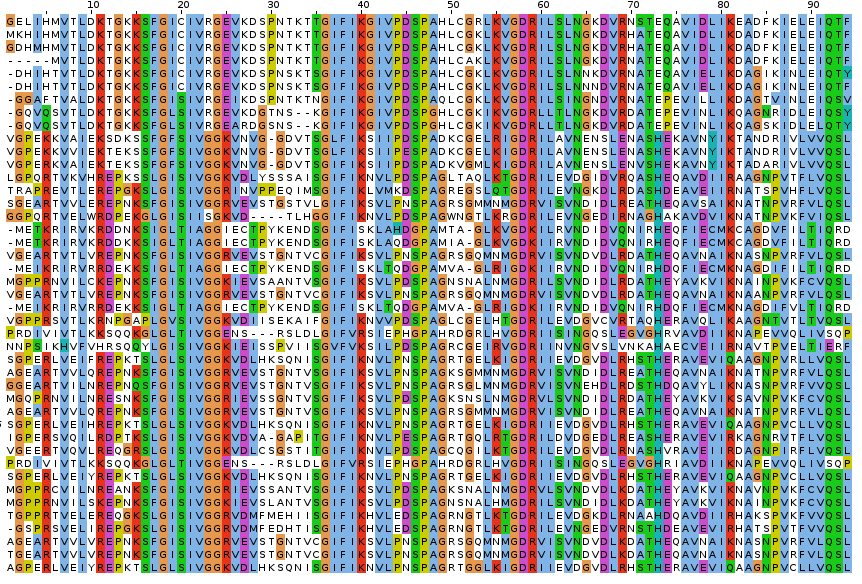
\includegraphics[width=17cm]{homologues/1IHJ.png} \\
     \end{tabular}
     \caption{L'alignement de notre sélection de séquences homologues à la protéine INAD (code PDB:1IHJ )}
\label{align_homo:INAD}
   \end{figure}

   \begin{figure}[t]
     \centering
     \begin{tabular}{c}
       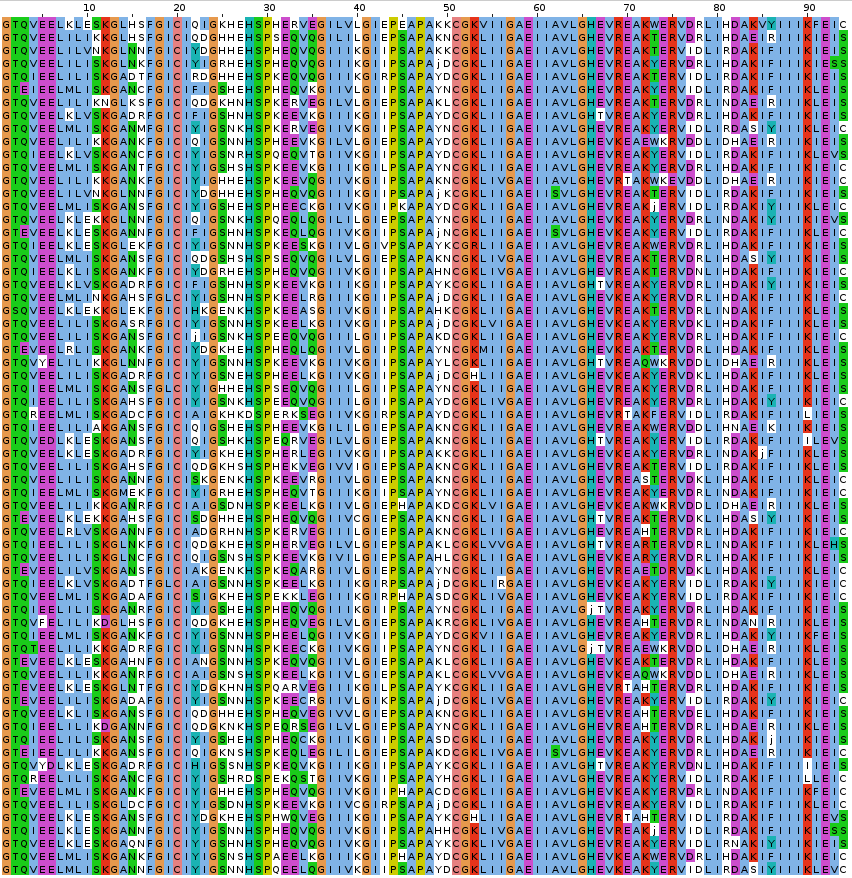
\includegraphics[width=17cm]{proteus/1IHJ.png} \\
     \end{tabular}
       \caption{Une sélection de séquences proteus, parmi les 10 000 séquences de meilleure énergie, obtenues avec le backbone de la protéine INAD (code PDB:1IHJ), modèle NEA}
\label{align_proteus:INAD}
   \end{figure}
\clearpage

   \begin{figure}[t]
     \centering
     \begin{tabular}{c}
       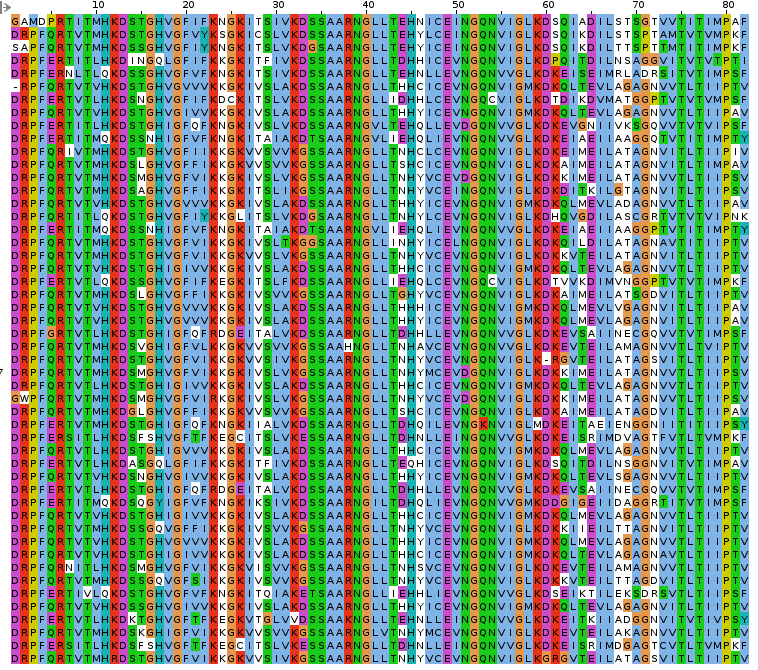
\includegraphics[width=17cm]{homologues/1R6J.png} \\
     \end{tabular}
     \caption{L'alignement de notre sélection de séquences homologues à la protéine Syntenin (code PDB 1R6J)}
\label{align_homo:Syntenin}
   \end{figure}

   \begin{figure}[t]
     \centering
     \begin{tabular}{c}
       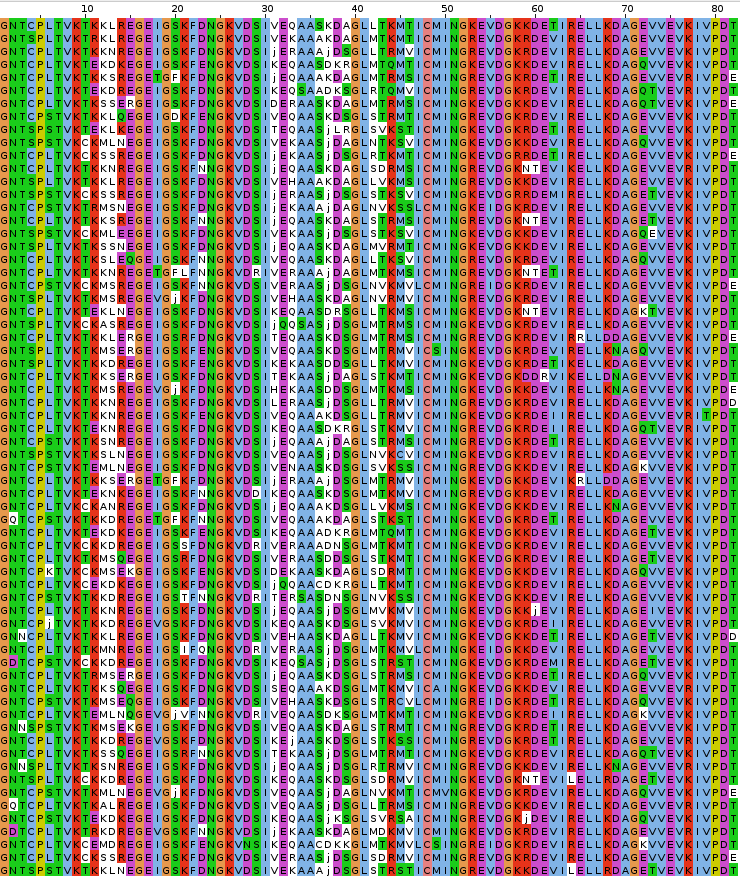
\includegraphics[width=17cm]{proteus/1R6J.png} \\
     \end{tabular}
       \caption{Une sélection de séquences proteus, parmi les 10 000 séquences de meilleure énergie, obtenues avec le backbone de la protéine Syntenin (code PDB:1R6J), modèle NEA}
\label{align_proteus:Syntenin}
   \end{figure}
\clearpage

   \begin{figure}[t]
     \centering
     \begin{tabular}{c}
       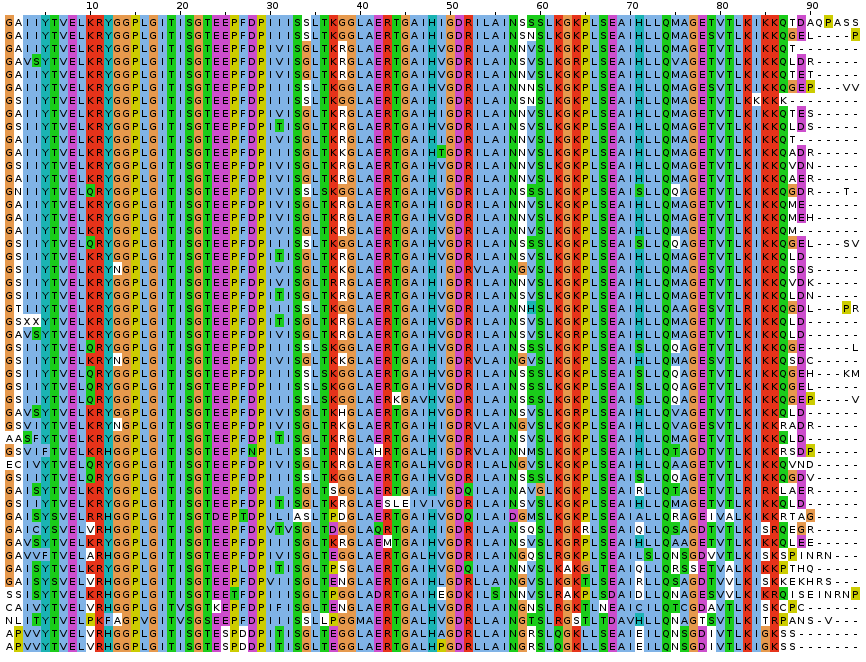
\includegraphics[width=17cm]{homologues/1N7E.png} \\
     \end{tabular}
     \caption{L'alignement de notre sélection de séquences homologues à la protéine GRIP (code PDB: 1N7E)}
\label{align_homo:GRIP}
   \end{figure}

   \begin{figure}[t]
     \centering
     \begin{tabular}{c}
       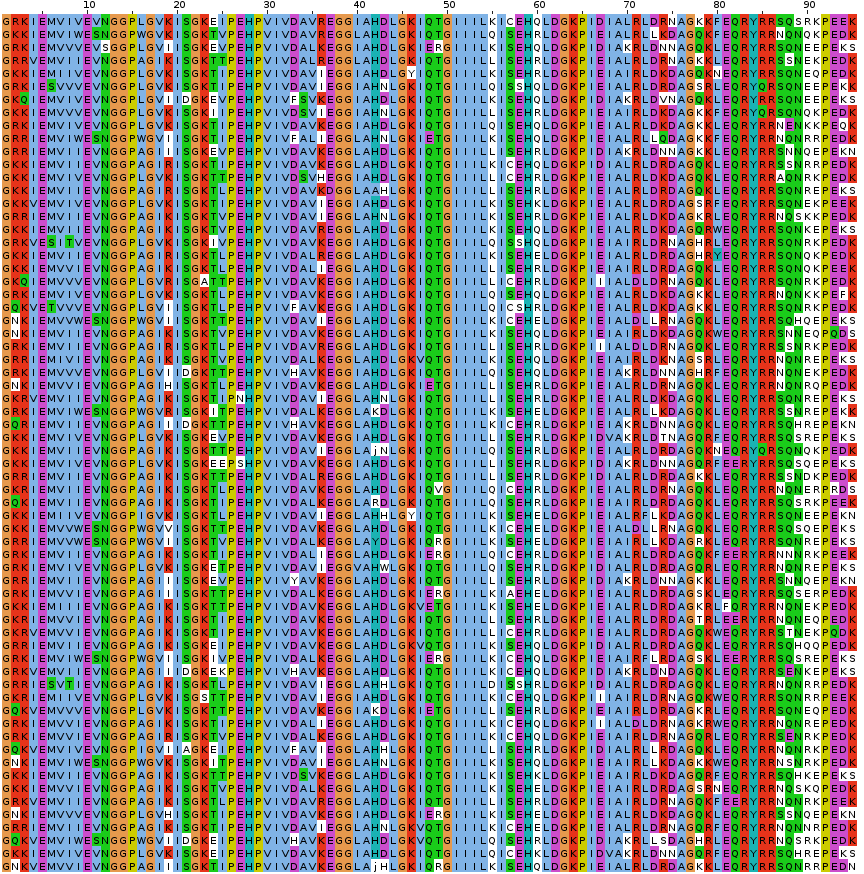
\includegraphics[width=17cm]{proteus/1N7E.png} \\
     \end{tabular}
       \caption{Une sélection de séquences proteus, parmi les 10 000 séquences de meilleure énergie, obtenues avec le backbone de la protéine GRIP (code PDB:1N7E), modèle NEA}
\label{align_proteus:GRIP}
   \end{figure}
\clearpage

   \begin{figure}[t]
     \centering
     \begin{tabular}{c}
       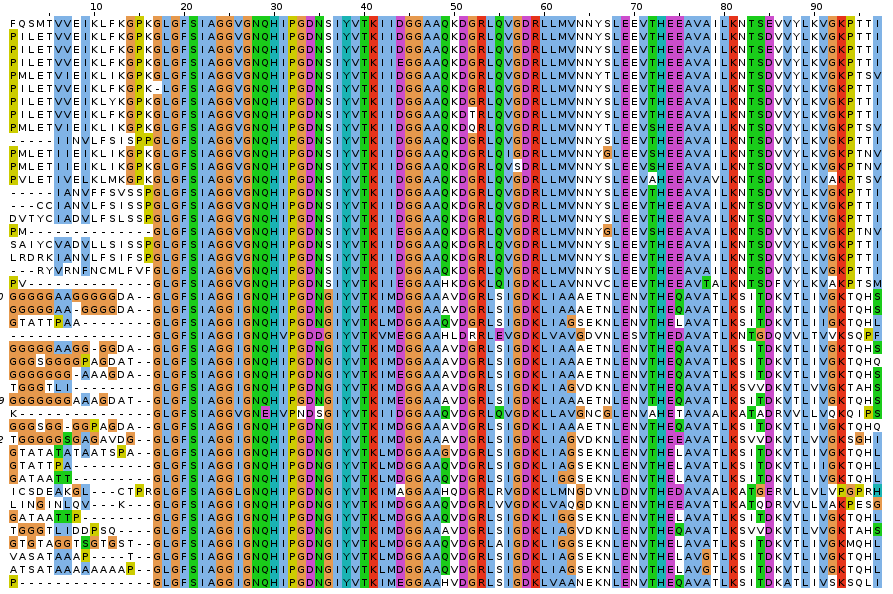
\includegraphics[width=17cm]{homologues/2BYG.png} \\
     \end{tabular}
     \caption{L'alignement de notre sélection de séquences homologues à la protéine DLG2 (code PDB 2BYG)}
\label{align_homo:DLG2}
   \end{figure}

   \begin{figure}[t]
     \centering
     \begin{tabular}{c}
       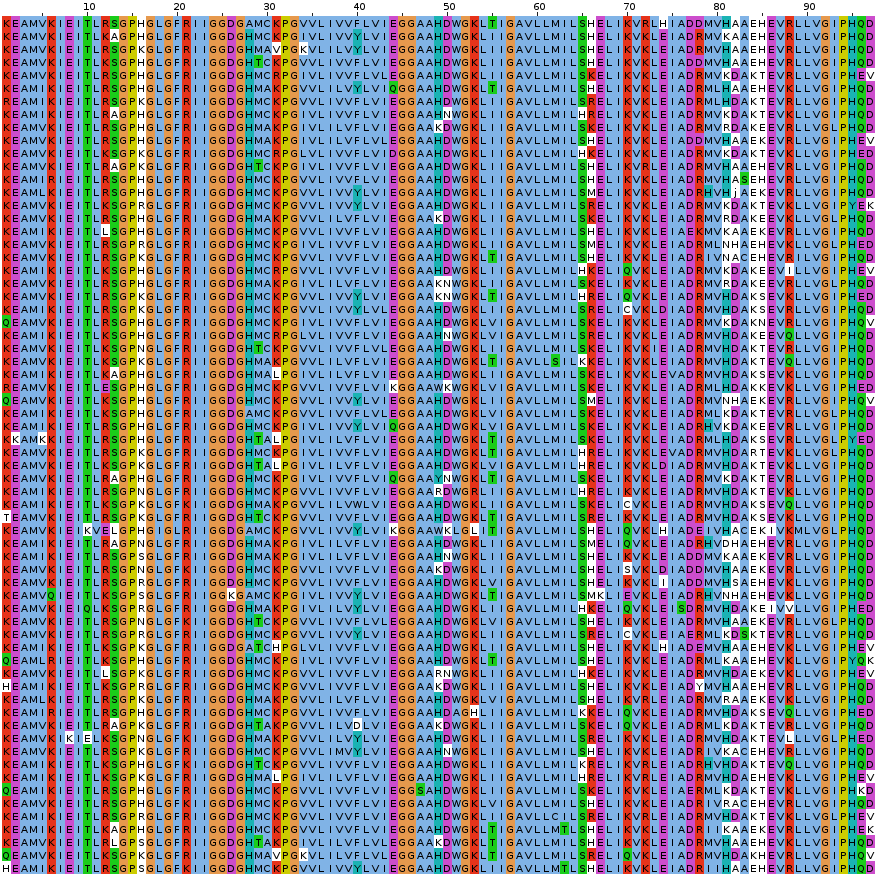
\includegraphics[width=17cm]{proteus/2BYG.png} \\
     \end{tabular}
       \caption{Une sélection de séquences proteus, parmi les 10 000 séquences de meilleure énergie, obtenues avec le backbone de la protéine DLG2 (code PDB 2BYG), modèle NEA}
\label{align_proteus:DLG2}
   \end{figure}
\clearpage

   \begin{figure}[t]
     \centering
     \begin{tabular}{c}
       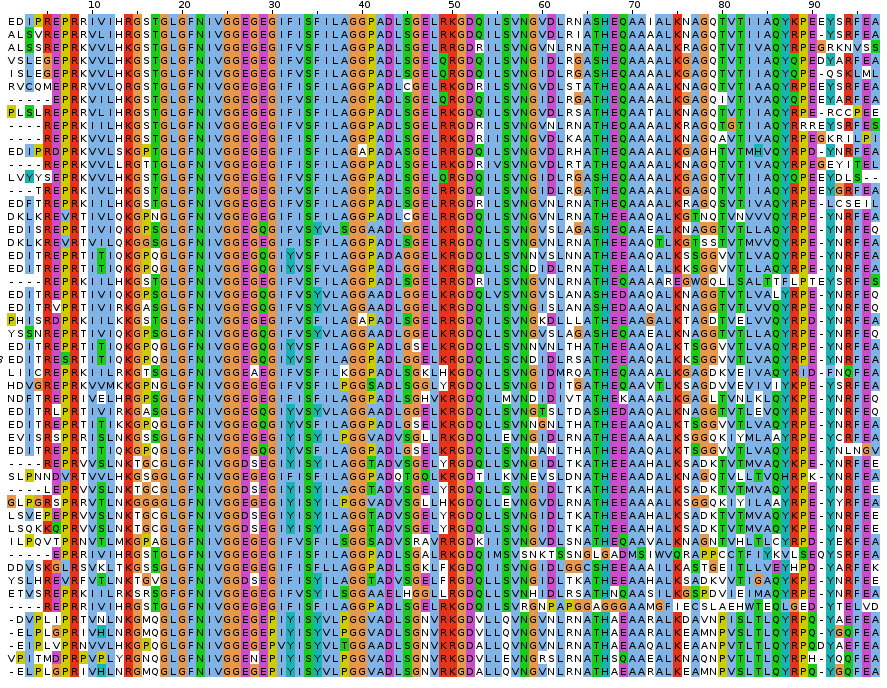
\includegraphics[width=17cm]{homologues/3K82.png} \\
     \end{tabular}
     \caption{L'alignement de notre sélection de séquences homologues à la protéine PSD95 (code PDB 3K82)}
\label{align_homo:PSD95}
   \end{figure}

   \begin{figure}[t]
     \centering
     \begin{tabular}{c}
       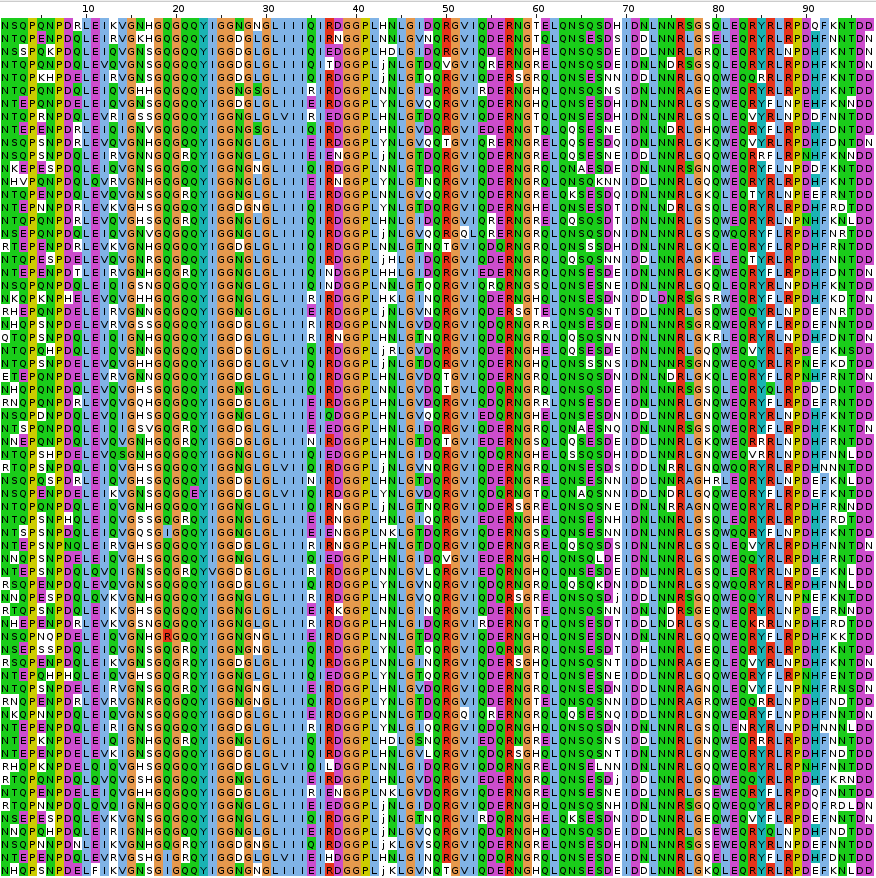
\includegraphics[width=17cm]{proteus/3K82.png} \\
     \end{tabular}
       \caption{Une sélection de séquences proteus, parmi les 10 000 séquences de meilleure énergie, obtenues avec le backbone de la protéine PSD95 (code PDB:3K82), modèle NEA}
\label{align_proteus:PSD95}
   \end{figure}
\clearpage

%   \begin{figure}[t]
%     \centering
%     \begin{tabular}{c}
%       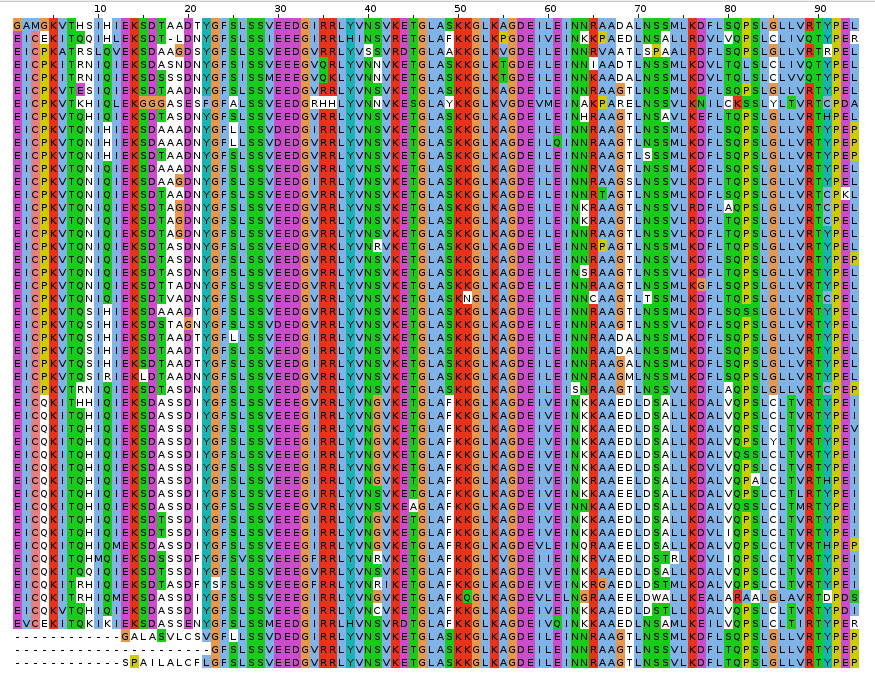
\includegraphics[width=17cm]{homologues/TIAM1.png} \\
%     \end{tabular}
%     \caption{L'aligmenent de notre sélection de séquences homologues à la protéine Tiam1 (code PDB )}
%\label{align_homo:Tiam1}
%   \end{figure}
%   
%   \begin{figure}[t]
%     \centering
%     \begin{tabular}{c}
%       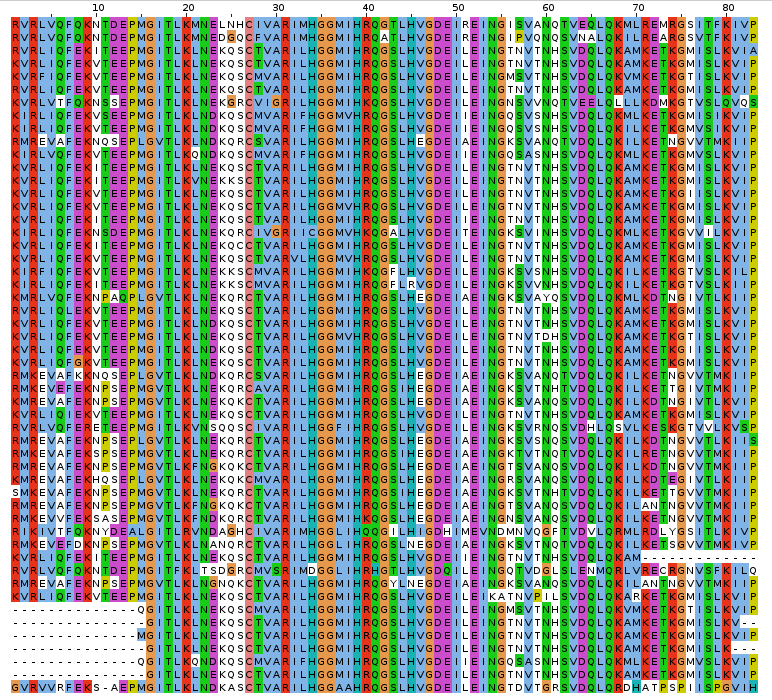
\includegraphics[width=17cm]{homologues/CASK.png} \\
%     \end{tabular}
%     \caption{L'aligmenent de notre sélection de séquences homologues à la protéine Cask (code PDB)}
%   \label{align_homo:CASK}
%   \end{figure}
%   
%\clearpage
%


\section{Séquences calculées}

\subsection{préparation}
Pour réaliser les calculs Monte-Carlo, Deux segments manquants dans le domaine Tiam1 (résidus 851-854 et 868-869) ont été construits en utilisant le programme Modeller (\cite{Modeller}). Le ligand peptidique a été retiré de la structure PDB avant de calculer la matrice d'énergie. les structures ont été préparées et les matrices d'énergie calculées à l'aide d'une procédure proposée dans des travaux précédents \cite{Schmidt08b,Schmidt09} et détaillée en \ref{sub:matrix}. 
 

\subsection{simulation Monte-Carlo}    

La production des séquences est réalisée avec Proteus \cite{Simonson13b}. Pour optimiser les énergies de références, les positions dans lesquels la séquence native comporte une glycine ou une proline conservent toujours leur type naturel et les positions mutables ne peuvent devenir ni Gly ni Pro. Pour optimiser les énergies de référence, nous sélectionnons, alternativement le long du backbone, une position pouvant muter, une position ne pouvant pas muter.

Dans tous les cas, des mutations sont produites au hasard, soumises uniquement à la fonction d'énergie MMGBSA qui entraîne la simulation. Les simulations Monte-Carlo utilisent des mouvements à une ou deux positions, où les rotamères,les types d'acides aminés ou les deux peuvent changer. Pour les mouvements à deux positions, la deuxième position est choisie parmi celles qui ont une énergie d'interaction significative avec la première pour au moins une conformation du couple formé de leur chaîne latérale respective (c'est à dire 10 kcal/mol ou plus). De plus, l'échantillonnage est amélioré par l'échange de répliques (REMC), où $8$ simulations MC de 500 millions de pas sont exécutées en parallèle , à différentes températures et avec échanges périodiques suivant le protocole REMCd qui est décrit en \ref{sub:REMCdetails}. Pour le calcul de fréquences, seules les séquences produites à la température $0.263$ sont retenues. 

\subsection{Génération de séquence Rosetta}

Des simulations Monte-Carlo sont également réalisées à l'aide du programme et de la fonction d'énergie Rosetta \cite{Baker06b}.Les simulations sont faites en utilisant la version 2015.38.58158 de la suite ( librement disponible en ligne ), en utilisant la commande:

\begin{verbatim}
fixbb -s Cask.pdb -resfile Cask.res -nstruct 10000 -ex1 -ex2 -linmem_ig 10
\end{verbatim} \normalsize


où les options ex1 et ex2 activent une recherche améliorée des rotamères pour les chaînes latérales enfouis. La dernière option correspond au calcul de l'énergie au cours de la recherche MC, et les paramètres par défaut sont utilisés pour les autres options.
Comme pour les simulations Proteus, les résidus Gly et Pro présents dans la protéine sauvage ne sont pas autorisé à muter, et les positions qui mutent ne peuvent pas le faire en Gly ou Pro. Des simulations sont exécutées pour chacun de nos domaines PDZ, jusqu'à obtenir 10 000 séquences uniques de faible énergie, ce qui correspond à des durées d'exécution d'environ 5 minutes par séquence sur un seul cœur d'un processeur Intel récent, pour un total de 10 heures par protéines en utilisant 80 cœurs. C'est tout à fait comparable au coût des calculs Proteus, en comptant le temps de calcul de la matrice d'énergie plus celui des simulations Monte-Carlo.


\subsection{Caractérisation des séquences calculées}

Les séquences calculées sont comparées à l'alignement Pfam pour la famille PDZ, en utilisant la matrice Blosum40 et une pénalité d'écart de -6. Cette matrice est appropriée pour comparer des homologies éloignées (les séquences CPD et celles de Pfam). Chaque séquence Pfam est également comparée à l'alignement Pfam, ce qui permet de comparer des séquences calculées et un couple de domaines PDZ naturels. Pour ces comparaisons Pfam/Pfam, si un domaine de test T fait partie de l'alignement, la comparaison T/T n'est pas prise en compte, pour être plus cohérent avec les comparaisons calculées/Pfam. L'alignement Pfam utilisée est le \og RP55 \fg ( voir la section \ref{subsection:Align_Pfam}). Les similitudes sont calculées pour les 14 résidus du cœur et pour l'ensemble des positions mutables de la protéine.

Les séquences calculées sont soumises à la bibliothèque de modèle de Markov Caché Superfamily \cite{Gough01,Wilson07}  qui tente de classer les séquences selon la base de données structurelle de protéines SCOP \cite{Andreeva04}, voir \ref{subsection:Superfamily} pour les détails. Le programme hmmscan est exécuté avec une E-value seuil d de $10^{-10}$. 

\section {Résultats du modèle NEA}
\label{sectionNEA} 
\subsection{optimisation du modèle de l'état déplié}

Nous optimisons les énergies de référence $E_t^r$ pour les six protéines de $\mathcal{S_1}$, en utilisant leurs homologues naturels pour définir les fréquences d'acides aminés cibles. La constante diélectrique de la protéine $\epsilon_p$ est fixé $8$. La méthode d'optimisation utilisée est la méthode linéaire voir (\ref{enumMeth}) avec 20 itérations avec la contrainte des classes et 20 itérations sans cette contrainte,l'optimisation ne se fait plus alors sur les six classes de type d'acide aminé , mais directement sur tous les types possibles. La fonction Proxy calculée sur les groupes de types converge autour les valeurs $0.06$, $0.07$ ( pour respectivement les énergies enfuies et exposées ) et pour les types les valeurs sont $0.08$ et $0.14$. Ce qui correspond à des variations  pour les $E_t^r$ inférieurs à $0,05 Kcal/mol$ pour tous les types d'acides aminés, ceci sur les 5 derniers cycles d'optimisation. Le tableau \ref{tab:RefEner6} donne les énergies de référence convergées, qui sont utilisées à la génération des séquences tests.

    \begin{table}[!htbp]
      \centering
      \caption{Les énergies de référence obtenues par l'optimisation sur 6 protéines.}
      \begin{tabular}{ccc}

        \toprule
        Type d'acides aminés & Pos. Enf. & Pos Exp. \\
        \cmidrule{1-3}

        ALA & 0.00     &  0,00     \\
        ARG & -28.29   &  -28.90   \\
        ASN & -5,94    &  -6,00    \\
        ASP & -9,19    &  -9,80    \\
        CYS & -1,04    &  -1,04    \\
        GLN & -4,72    &  -4,78    \\
        GLU & -7,90    &  -8,51    \\
        HID & 11.96    &  12,39    \\
        HIE & 11,43    &  11,85    \\
        HIP & 14,53    &  14,96    \\
        ILE & 4,72     &  2,11     \\
        LEU & 1,17     &  -1,44    \\
        LYS & -4,56    &  -4,47    \\
        MET & -2,78    &  -3,54    \\
        PHE & -0,37    &  -2,55    \\
        SER & -3,73    &  -2,80    \\
        THR & -3,82    &  -3,82    \\
        TRP & -1,61    &  -3,79    \\
        TYR & -4,20    &  -6,10    \\
        VAL & 0,83     &  -1,77    \\

        \bottomrule
      \end{tabular}      

\label{tab:RefEner6}      
    \end{table}

Le tableau \ref{Tab:FreqAA6} compare les fréquences d'acide aminé des homologues naturels avec les fréquences d'acide aminé des séquences calculées. La population théorique des différentes classes d'acide aminé a bien rejoint l'expérience, avec des écarts de moins de un pourcent dans la majorité des cas, pour les positions exposées et pour les positions enfuies, seulement deux classes ont des écarts de plus de 2\% (2,1 et 2,6 pour Lys et Arg aux positions exposées). L'accord entre les types d'acide aminé est aussi bon avec pour les mauvais cas, deux écarts à plus de 2\%  qui correspondent au deux plus mauvaises classes. Pendant les 20 premiers cycles d'optimisation,la distribution des fréquences intra classe dépend par construction du $\delta E_t^r$ défini dans pour chaque classe, qui ont était calculés par mécanique moléculaire (voir méthodes). La seconde série de 20 itérations permet l'ajustement de ces valeurs. 
    
\begin{table}
  \centering
\caption{Les compositions en acide aminé (\%) des séquences expérimentales et Proteus après optimisation des $E_t^s$. Les différences entre expérimentale et théorique sont indiquées entre parenthèses.Les types d'acides aminés sont rassemblés selon les groupes d'optimisations.}
\begin{tabular}{lcccc|cccc}
\hline
 & \multicolumn{4}{c}{Experimentale}& \multicolumn{4}{c}{Proteus}\\
Res & \multicolumn{2}{c}{Enfoui} & \multicolumn{2}{c}{Exposé} & \multicolumn{2}{c}{Enfoui} & \multicolumn{2}{c}{Exposé} \\
\hline
ALA&10.9&\multirow{3}{*}{16,9}&4,6&\multirow{3}{*}{13,4}&11,1&\multirow{2}{*}{17,0}&4,4&\multirow{2}{*}{12,0}\\
CYS&1.3&&0.5&&0.0&\multirow{2}{*}{(0.1)}&0.3&\multirow{2}{*}{(-1,4)}\\
THR&4.7&&8.3&&5.9&&7.3\\
\hline
ASP&4.3&\multirow{2}{*}{6,8}&6,0&\multirow{2}{*}{17,9}&4,5&\multirow{1}{*}{6,7}&5,6&\multirow{1}{*}{16,7}\\
GLU&2.5&&11.9&&2.2&(-0,1)&11,1&(-1,2)\\
\hline                          
ASN&2.6&\multirow{2}{*}{4,7}&6,7&\multirow{2}{*}{12,2}&2,5&\multirow{1}{*}{4,7}&7,5&\multirow{1}{*}{14,0}\\
GLN&2.1&&5.5&&2.2&(0,0)&6,5&(1,8)\\
\hline                                                                                       
HIP&1.2&\multirow{3}{*}{1,2}&5,0&\multirow{3}{*}{5,0}&1,0&\multirow{2}{*}{1,1}&5,2&\multirow{2}{*}{5,6}\\
HIE&0.0&&0.0&&0.1&\multirow{2}{*}{(-0,1)}&0.4&\multirow{2}{*}{(0.6)}\\
HID&0.0&&0.0&&0.0&&0.0\\
\hline                                                                                  
ILE&16.0&\multirow{3}{*}{50.7}&4.2&\multirow{3}{*}{14.0}&16.9&\multirow{2}{*}{52.1}&4.1&\multirow{2}{*}{14.0}\\
VAL&16.5&&5.4&&16.7&\multirow{2}{*}{(1.4)}&5.6&\multirow{2}{*}{(0.0)}\\
LEU&18.2&&4.4&&18.5&&4.3\\
\hline                                                                              
\multirow{2}{*}{LYS}&\multirow{2}{*}{2,5}&\multirow{2}{*}{2,5}&\multirow{2}{*}{10,9}&\multirow{2}{*}{10,9}&\multirow{2}{*}{1,5}&1,5&\multirow{2}{*}{13,0}&13,0\\
&&&&&&(-1,0)&&(2.1)\\
\hline                                                                        
\multirow{2}{*}{MET}&\multirow{2}{*}{0,9}&\multirow{2}{*}{0,9}&\multirow{2}{*}{1,5}&\multirow{2}{*}{1,5}&\multirow{2}{*}{1,6}&1,6&\multirow{2}{*}{1,4}&1,4\\
&&&&&&(0,7)&&(-0.1)\\
\hline                                                                         
\multirow{2}{*}{ARG}&\multirow{2}{*}{2,8}&\multirow{2}{*}{2,8}&\multirow{2}{*}{8,7}&\multirow{2}{*}{8,7}&\multirow{2}{*}{2,5}&2,5&\multirow{2}{*}{6,1}&6,1\\
&&&&&&(-0,3)&&(-2.6)\\
\hline                                                                                  
\multirow{2}{*}{SER} &\multirow{2}{*}{5,3}&\multirow{2}{*}{5,3}&\multirow{2}{*}{7,6}&\multirow{2}{*}{7,6}&\multirow{2}{*}{4,3}&4,3&\multirow{2}{*}{8,7}&8,7\\
&&&&&&(-1,0)&&(1.1)\\
\hline                                                         
PHE      &4,1&\multirow{2}{*}{4,1}&2,4&\multirow{2}{*}{2,4}&4,5&\multirow{1}{*}{4,6}&2,1&\multirow{1}{*}{2,1}\\
TRP&0.0&&0.0&&0.1&(0,5)&0,0&(-0,3)\\
\hline                                                                                                                                                                                   
\multirow{2}{*}{TYR}&\multirow{2}{*}{2,6}&\multirow{2}{*}{2,6}&\multirow{2}{*}{1,2}&\multirow{2}{*}{1,2}&\multirow{2}{*}{2,2}&2,2&\multirow{2}{*}{0,4}&0,4\\
&&&&&&(-0,4)&&(-0.8)\\
\hline                                                                                                                                                                            
GLY&0.8&\multirow{2}{*}{0,9}&3,1&\multirow{2}{*}{4,9}&0,0&\multirow{1}{*}{0,0}&0,0&\multirow{1}{*}{0,0}\\
PRO&0.1&&1.8&&0.0&(-0,9)&0,0&(-4,9)\\
\hline
\end{tabular}
\label{Tab:FreqAA6}
\end{table}



\subsection{Tests de reconnaissance de famille}
À partir de nos énergies optimisées, nous générons des séquences pour chaque protéine.
Les simulations Proteus utilisent l'algorithme REMC avec huit répliques (ou marcheurs) et 750 millions de pas par réplique, et des énergies thermiques kT  qui varient de 0,125 à 3 kcal/mol. Il s'agit du protocole REMCd détaillé en \ref{sub:REMCdetails}. Toutes les positions sont autorisées à muter librement vers tous les types d'acides aminés exceptés Gly et Pro. Les simulations ont été faites avec la fonction d'énergie MMGBSA, sans aucune introduction de biais vers les séquences naturelles ni aucune limite sur le nombre de mutations. Les 10 000 séquences avec les énergies les plus faibles parmi celles échantillonnées par au moins une des marcheurs MC sont retenues pour l'analyse. De la même façon, 10 000 séquences produites par Rosetta ont était retenues. Ces séquences sont analysées par les outils de reconnaissance de repliement \og Superfamily \fg (voir \ref{{subsection:Superfamily}}). Avec une constante diélectrique de 8, nous avons obtenu un pourcentage élevé de séquences correctement associées à la famille et superfamille PDZ: 100\% pour NHREF, INAD,GRIP et DLG2 , 99\%  pour Syntenin , seule PSD95 donne un score relativement mauvais de 47\% pour la famille et 50\% pour la superfamille. Les E-values sont inférieures à $10^{-3}$ pour les affectations à la famille. Ces valeurs sont semblables à celles obtenues par Rosetta pour les cinq premiers cas, par contre l'affectation à la superfamille est meilleure pour Rosetta avec des E-values compris entre $3.7$ $10^{-23}$ et $1.3$ $10^{-9}$, alors que Proteus obtient des E-values compris entre $4$ $10^{-4}$ et $2$ $10^{-12}$ si l'on exclut PSD95. Les détails sont présentés aux tables \ref{tab:superfamily_model_B6} et \ref{tab:superfamily_bestRE}.


\begin{table}[h]
  
  \begin{tabular}{cccccc}
    
    \toprule
    Protein & Match/seq & Superfamily & Superfamily & Family & Family \\
            & size      & Evalue      & success     & Evalue & success\\
    \cmidrule{1-6}
    NHREF  & 81/91 &     2.00 $10^{-12}$ & 10000  & 9.97 $10^{-3}$ & 10000  \\
    INAD  & 84/94 &      4.80 $10^{-11}$ & 10000  & 2.83 $10^{-3}$ & 10000  \\
    GRIP  & 82/95 &      4.73 $10^{-8}$  & 10000  & 5.56 $10^{-3}$ & 10000  \\
    Syntenin  & 63/91 &  4.01 $10^{-4}$  &  9999  & 1.05 $10^{-2}$ &  9999  \\
    DLG2  & 84/97 &      3.82 $10^{-10}$ & 10000  & 3.75 $10^{-3}$ & 10000  \\
    PSD95  & 46/97 &     7.65 $10^{-1}$  &  5029  & 4.06 $10^{-2}$ &  4719  \\

    \bottomrule        
  \end{tabular}   
  \caption{Résultats Superfamily pour les séquences Proteus avec le modèle NEA.}   
  \label{tab:superfamily_model_B6}       
\end{table}

\begin{table}[h]

  \begin{tabular}{cccccc}
    
    \toprule
    Protein & Match/seq & Superfamily & Superfamily & Family & Family \\
            & size      & Evalue      & success     & Evalue & success\\
    \cmidrule{1-6}
    NHREF    & 79/91   &    1.3 $10^{-13}$ & 10000 & 2.2 $10^{-3}$ & 10000 \\
    INAD     & 85/94   &    7.4 $10^{-14}$ & 10000 & 3.7 $10^{-3}$ & 10000 \\
    GRIP     & 84/95   &    2.2 $10^{-10}$ & 10000 & 1.2 $10^{-3}$ & 10000 \\
    Syntenin & 76/82   &    7.3 $10^{-13}$ & 10 000 & 1,8 $10^{-3}$ & 10 000 \\
    DLG2     & 86/97   &    1.3 $10^{-9}$  & 10 000 & 9,6 $10^{-4}$ & 10 000 \\
    PSD95    & 90/97   &    3.7 $10^{-23}$ & 10 000 & 5,2 $10^{-4}$ & 10 000 \\
    \bottomrule        
  \end{tabular}   
  \caption{Résultats Superfamily pour les séquences Rosetta}   
  \label{tab:superfamily_bestRE}       
\end{table}


\subsection{Séquences et diversité de séquences}
Une sélection des meilleures séquences calculées par Proteus, au sens de l'énergie, pour le sous-ensemble de 6 protéines est montrée aux figures \ref{align_proteus:NHREF} pour NHREF, \ref{align_proteus:INAD} pour INAD ,\ref{align_proteus:Syntenin} pour Syntenin, \ref{align_proteus:GRIP} pour GRIP, \ref{align_proteus:DLG2} pour DLG2 , \ref{align_proteus:PSD95} et pour PSD95. Les homologues naturels sont présentés aux figures \ref{align_homo:NHREF} pour NHREF, \ref{align_homo:INAD} pour INAD, \ref{align_homo:Syntenin} pour Syntenin ,\ref{align_homo:GRIP} pour GRIP ,\ref{align_homo:DLG2} pour DLG2 et \ref{align_homo:PSD95} pour PSD95. La coloration est celle de clustalX implémenté dans Jalview \cite\{Jalview}. Comme cela a été établi dans de nombreuses études de CPD antérieures (30,72), l'accord avec l'expérience pour les positions du cœur est très bon, alors que l'accord en ce qui concerne les résidus de surface est nettement plus faible. La diversité des séquences naturelles et des séquences calculées est caractérisée par la moyenne sur la séquence de l'exponentielle de l'entropie résiduelle (voir \ref{subsection:Entropie}).Comme référence nous utilisons l'ensemble Pfam Seed qui est constitué d'un sous-ensemble représentatif des domaines PDZ naturels (\ref{subsection:AlignPfam}).

L'entropie est calculée aux positions de chaque protéine. La diversité des séquences Rosetta est légèrement meilleure avec des valeurs comprises entre $1.4$ et $1.68$ alors que celles de Proteus sont comprises $1.24$ et $1.55$ tandis que la diversité de Pfam Seed se situe  a une entropie moyenne de $3,11$. Le regroupement des séquences de NHREF,INAD,GRIP,Syntenin,DLG2 et PSD95 calculés  donne une entropie de $2,88$ avec Rosetta et $2.42$ avec Proteus. Ce qui indique que seulement six géométries de backbone ne peuvent pas atteindre les mêmes niveaux de diversités que l'ensemble Seed conçu pour caractériser la diversité des domaines PDZ et notamment la diversité de leur squelette.


    \begin{table}[!htbp]
      \centering

      \begin{tabular}{ccccc}

        \toprule
        Protein & Proteus & Rosetta & Pfam seed \\
        \cmidrule{1-4}
        NHREF  & 1.38 & 1.45 & 3.15  \\
        INAD  & 1.37 & 1.55 & 3.06  \\
        GRIP  & 1.33 & 1.44 & 3.09  \\
        Syntenin  & 1.39 & 1.43 & 3.03  \\
        DLG2  & 1,24 & 1,57 & 3,11  \\
        PSD95  & 1,27 & 1,40 & 3,15  \\
        6prots & 2,42  & 2,88 &    \\
        \cmidrule{1-5}
        CASK  & 1.55 & 1.68 & 3.15  \\
        TIAM1 & 1,22 & 1,57 & 3,15  \\

        \bottomrule

      \end{tabular}      
      \caption{Moyenne de l'exponentielle de l'entropie sur les ensembles des positions des protéines}
\label{tab:Entropie_PDZ}      
    \end{table}

        
\subsection{Scores de similarité Blosum}

Les scores de similarité Blosum40 entre les séquences calculées et les séquences naturelles sur l'ensemble des positions sont globalement faibles (voir la figure \ref{fig:similNEAfull}).les similitudes Proteus et Rosetta se chevauchent au pied du somment des scores naturels pour NHREF INAD, GRIP et DLG2 avec des valeurs Proteus en retrait  par rapport à celles de Rosetta de quelques dixièmes de points, moins de 20 pour NHREF, mais près de 50 pour Syntenin. Les résultats Proteus pour PSD95 sont beaucoup moins bons que ceux de Rosetta avec un écart moyen de plus de 70. En ce qui concerne les résidus du cœur, montrés à la figure  \ref{fig:similNEAcore} la similitude des séquences calculées avec les séquences naturelles est beaucoup plus forte, avec beaucoup de séquences Proteus avec des scores à plus de 30 pour NHREF,INAD et DLG2. Proteus fait jeu égal avec Rosetta sur NHREF et Syntenin, et est globalement meilleur sur INAD et DLG2, et moins bon sur GRIP et PSD95. 


   \begin{figure}[t]
     \centering
     \begin{tabular}{cc} 
       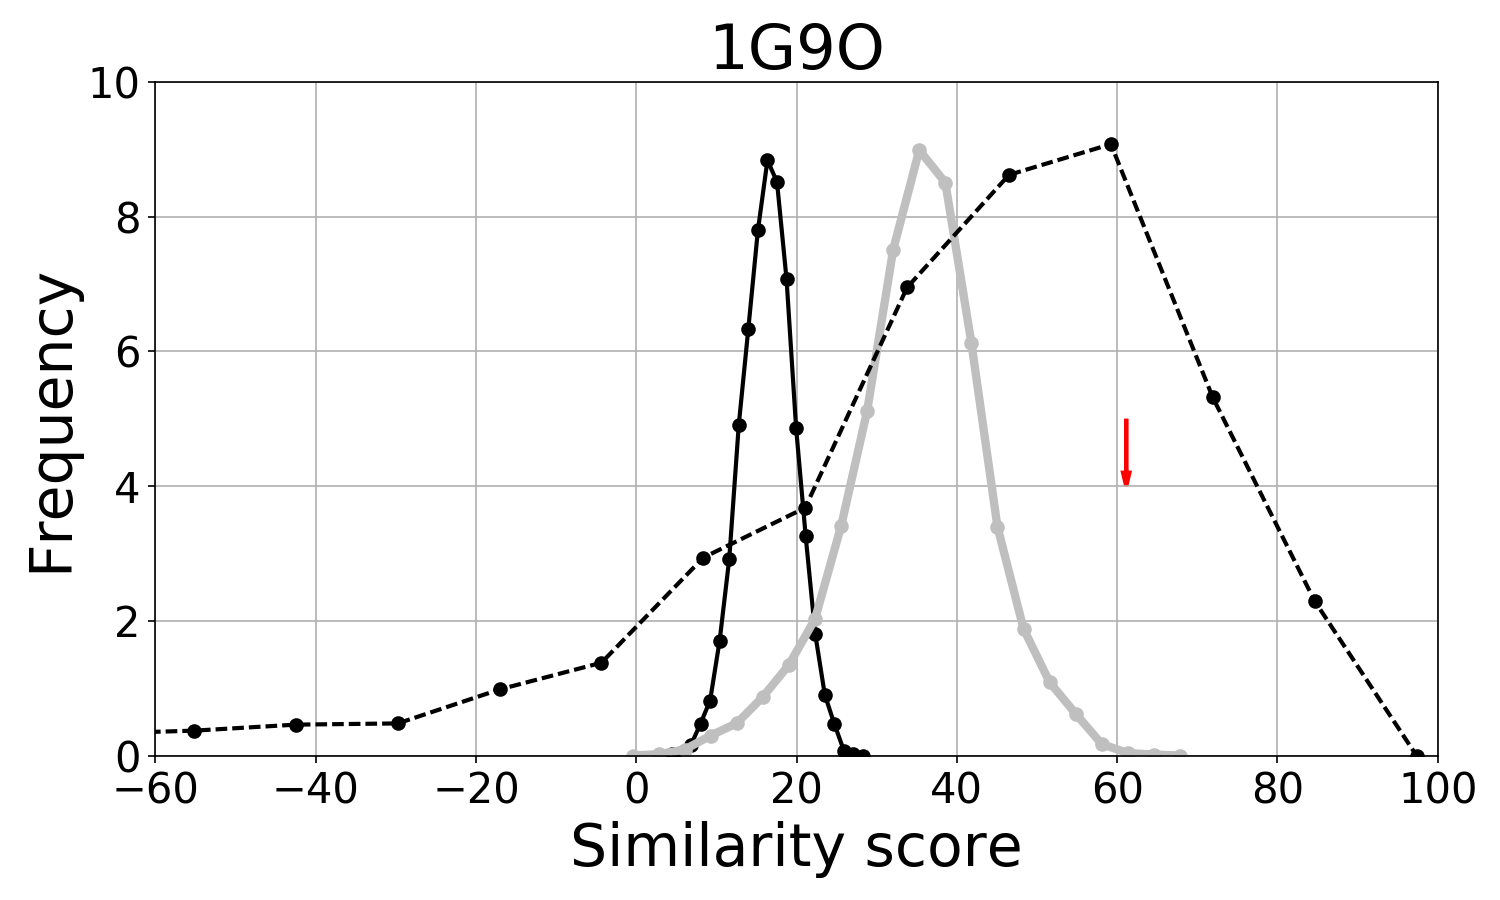
\includegraphics[width=8.4cm]{modelB6+/1G9O_simil_full.png} &
       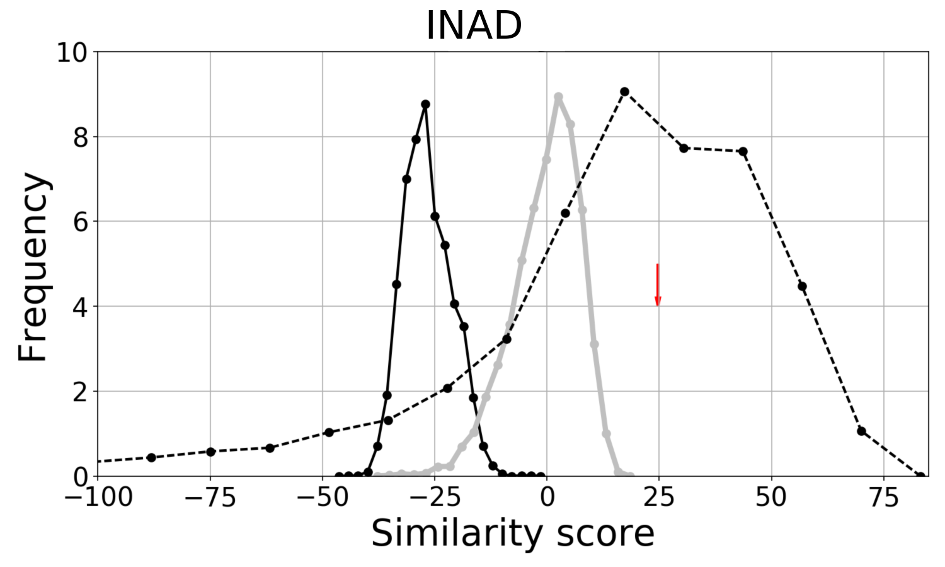
\includegraphics[width=8.4cm]{modelB6+/1IHJ_simil_full.png} \\
       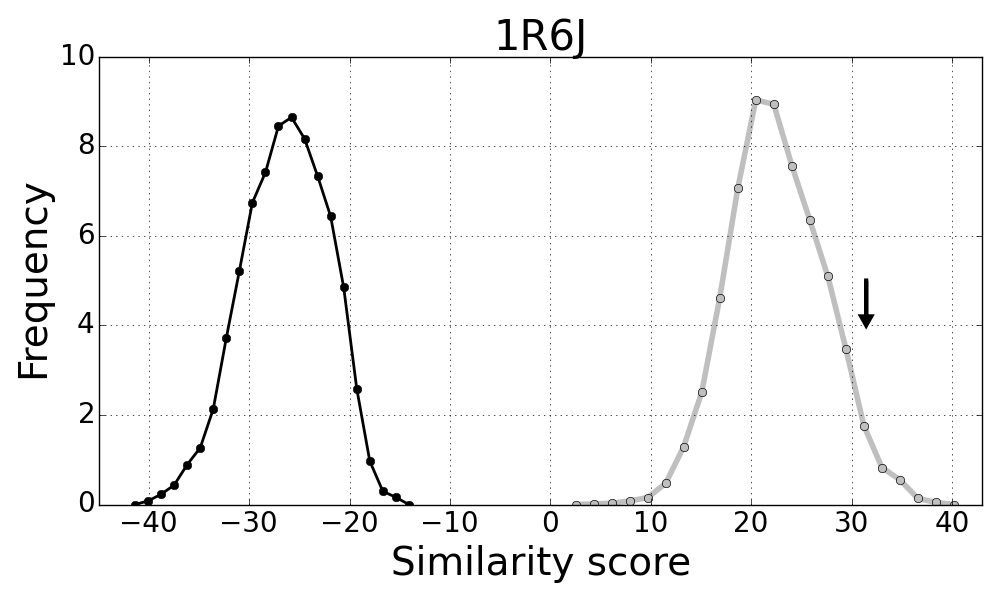
\includegraphics[width=8.4cm]{modelB6+/1R6J_simil_full.png} &
       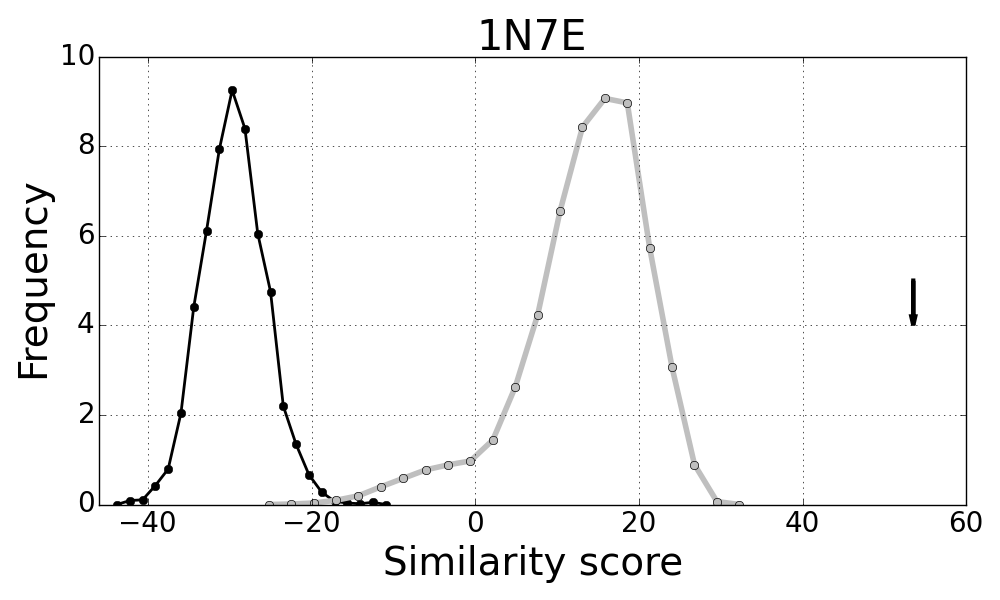
\includegraphics[width=8.4cm]{modelB6+/1N7E_simil_full.png} \\
       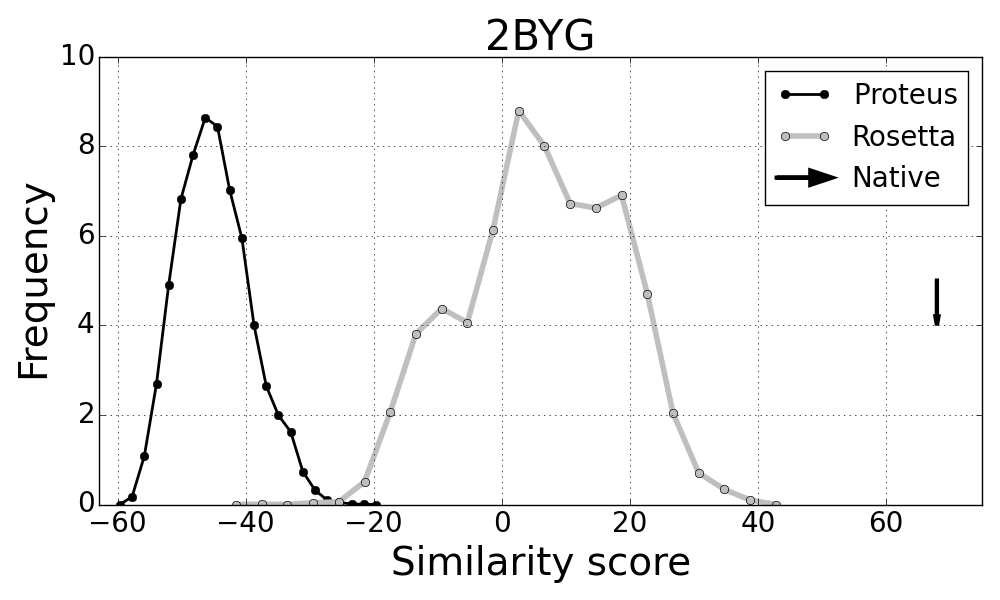
\includegraphics[width=8.4cm]{modelB6+/2BYG_simil_full.png} &
       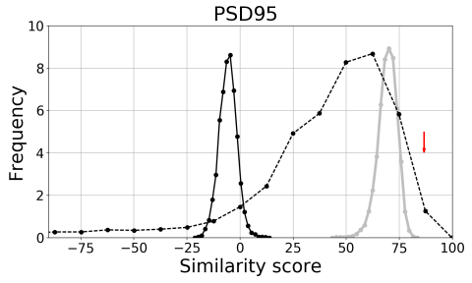
\includegraphics[width=8.4cm]{modelB6+/3K82_simil_full.png} \\
     \end{tabular}
  \caption{Similarité des séquences des 6 protéines produites par Proteus et Rosetta à l'alignement Pfam RP55, sur l'ensemble des positions.}
\label{fig:similNEAfull}
   \end{figure}



   \begin{figure}[t]
     \centering
     \begin{tabular}{cc} 
       \includegraphics[width=8.4cm]{modelB6+/1G9O_simil_core.png} &
       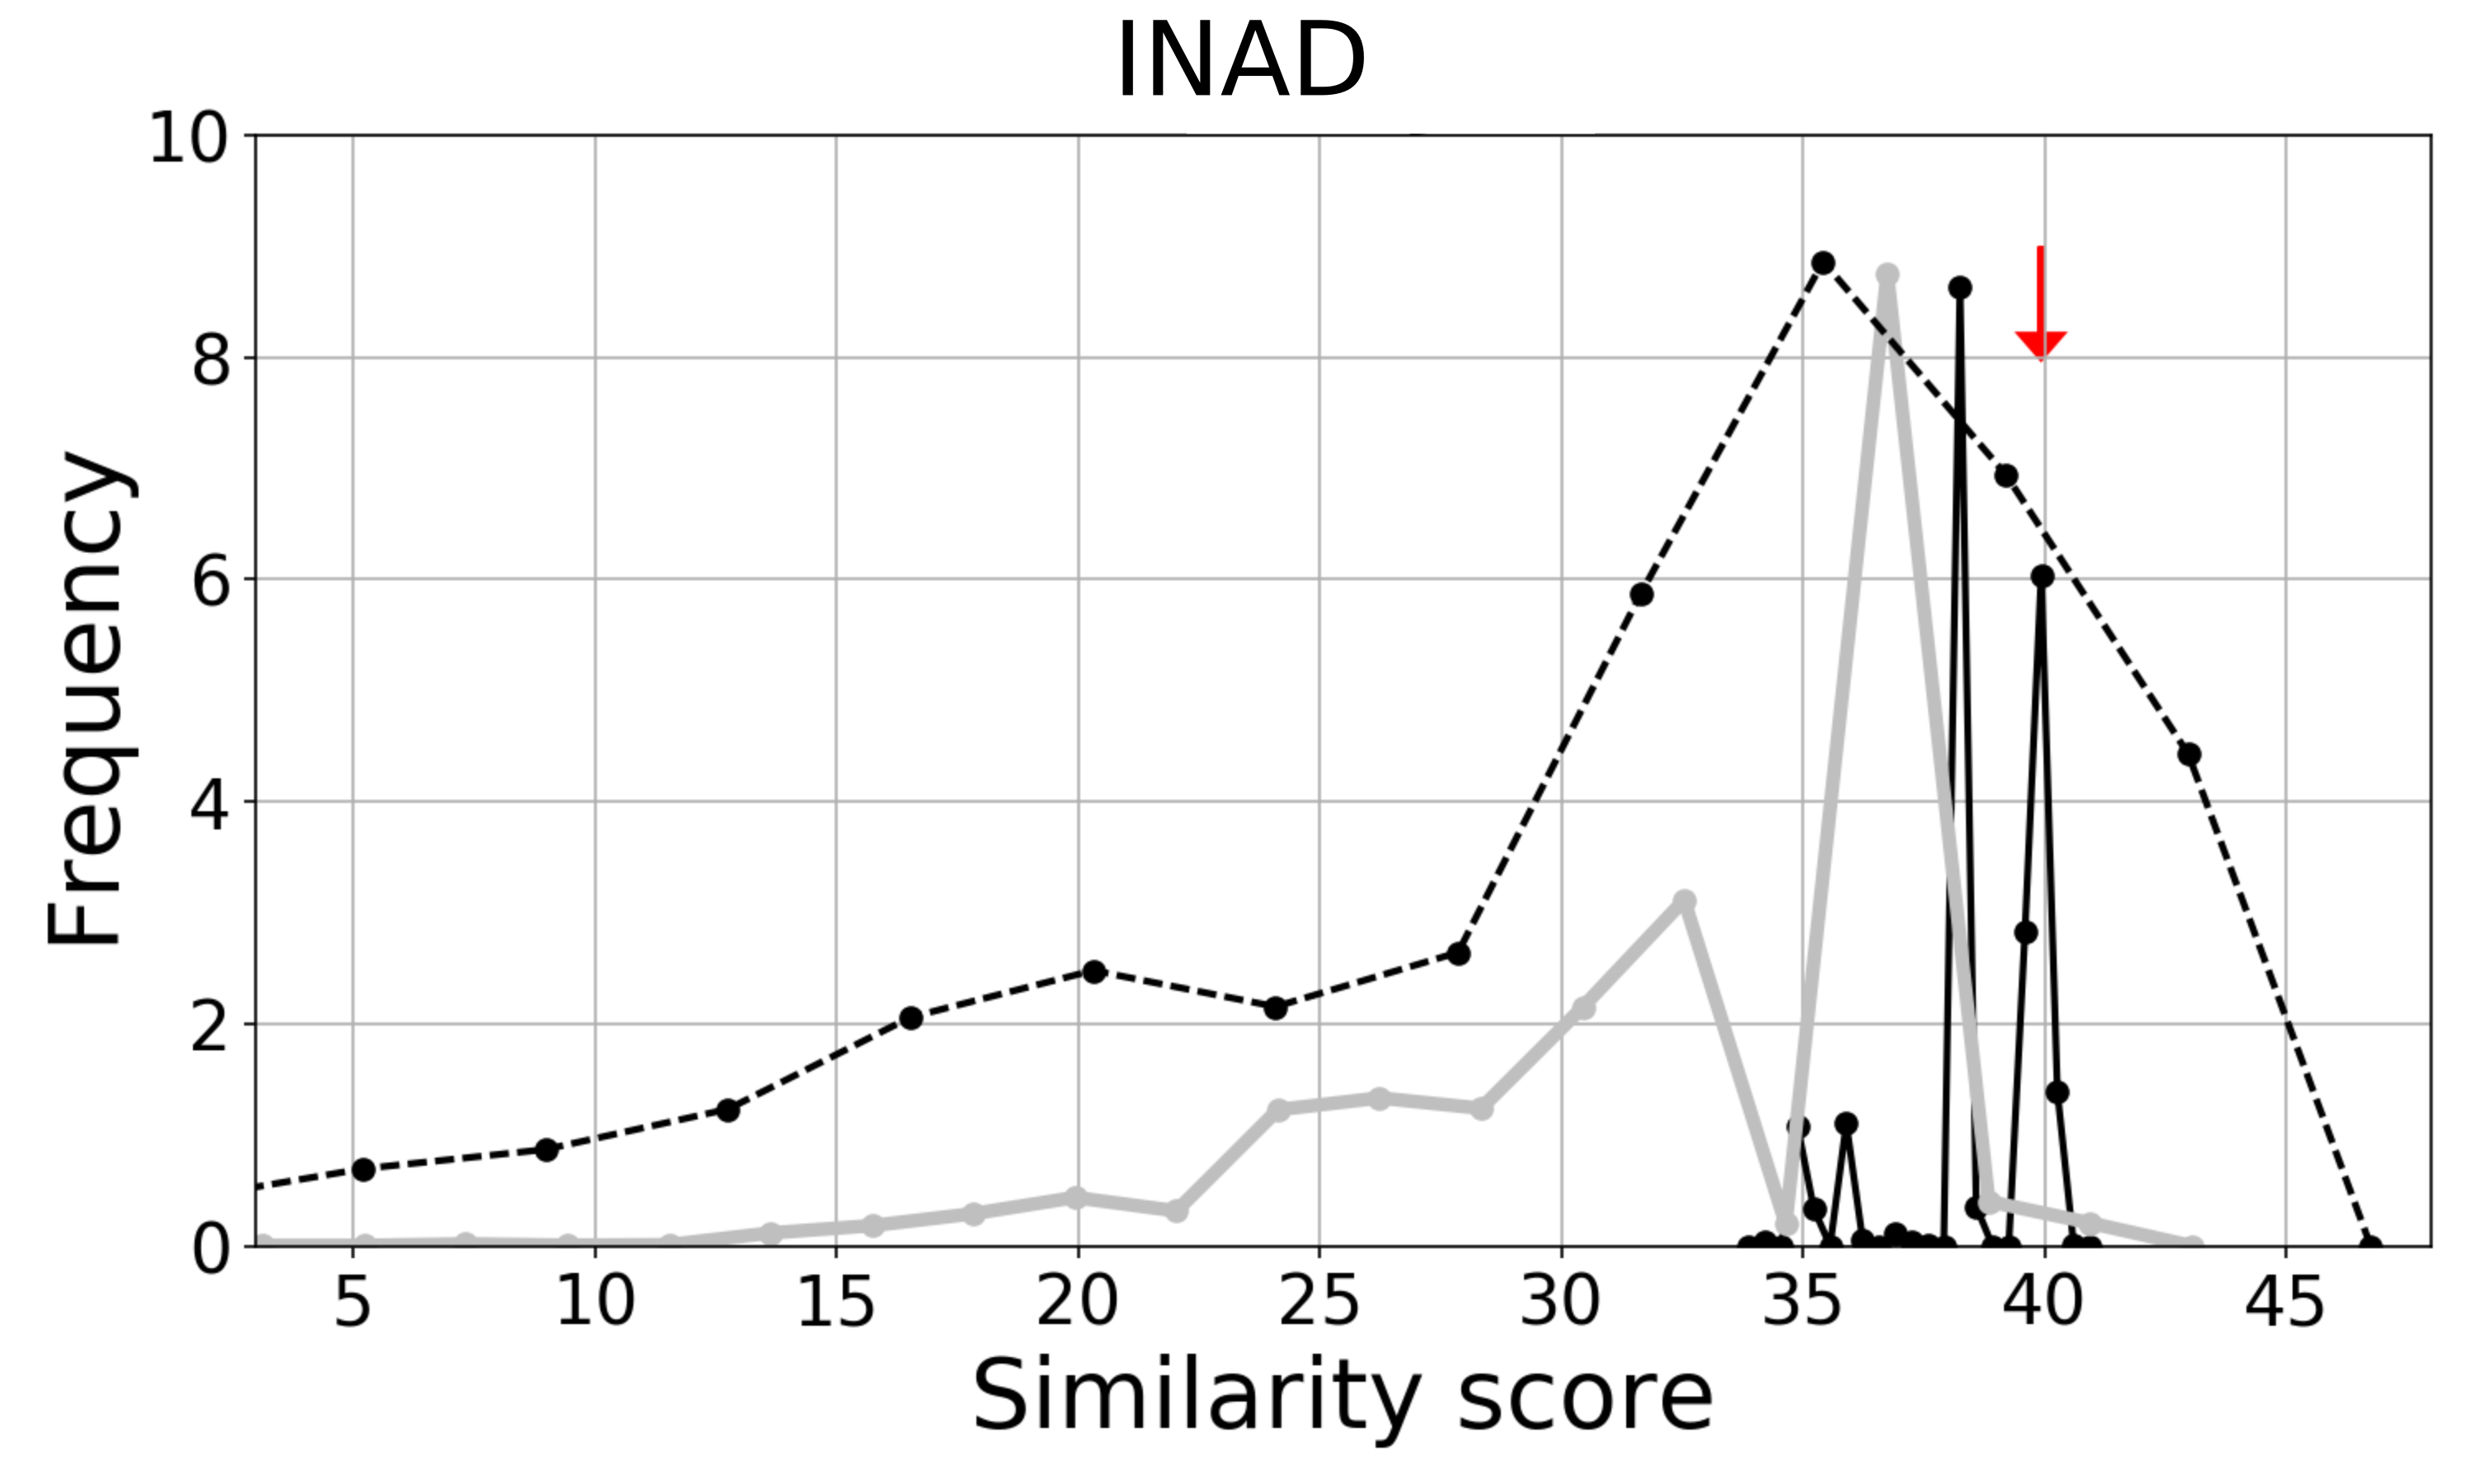
\includegraphics[width=8.4cm]{modelB6+/1IHJ_simil_core.png} \\
       \includegraphics[width=8.4cm]{modelB6+/1R6J_simil_core.png} &
       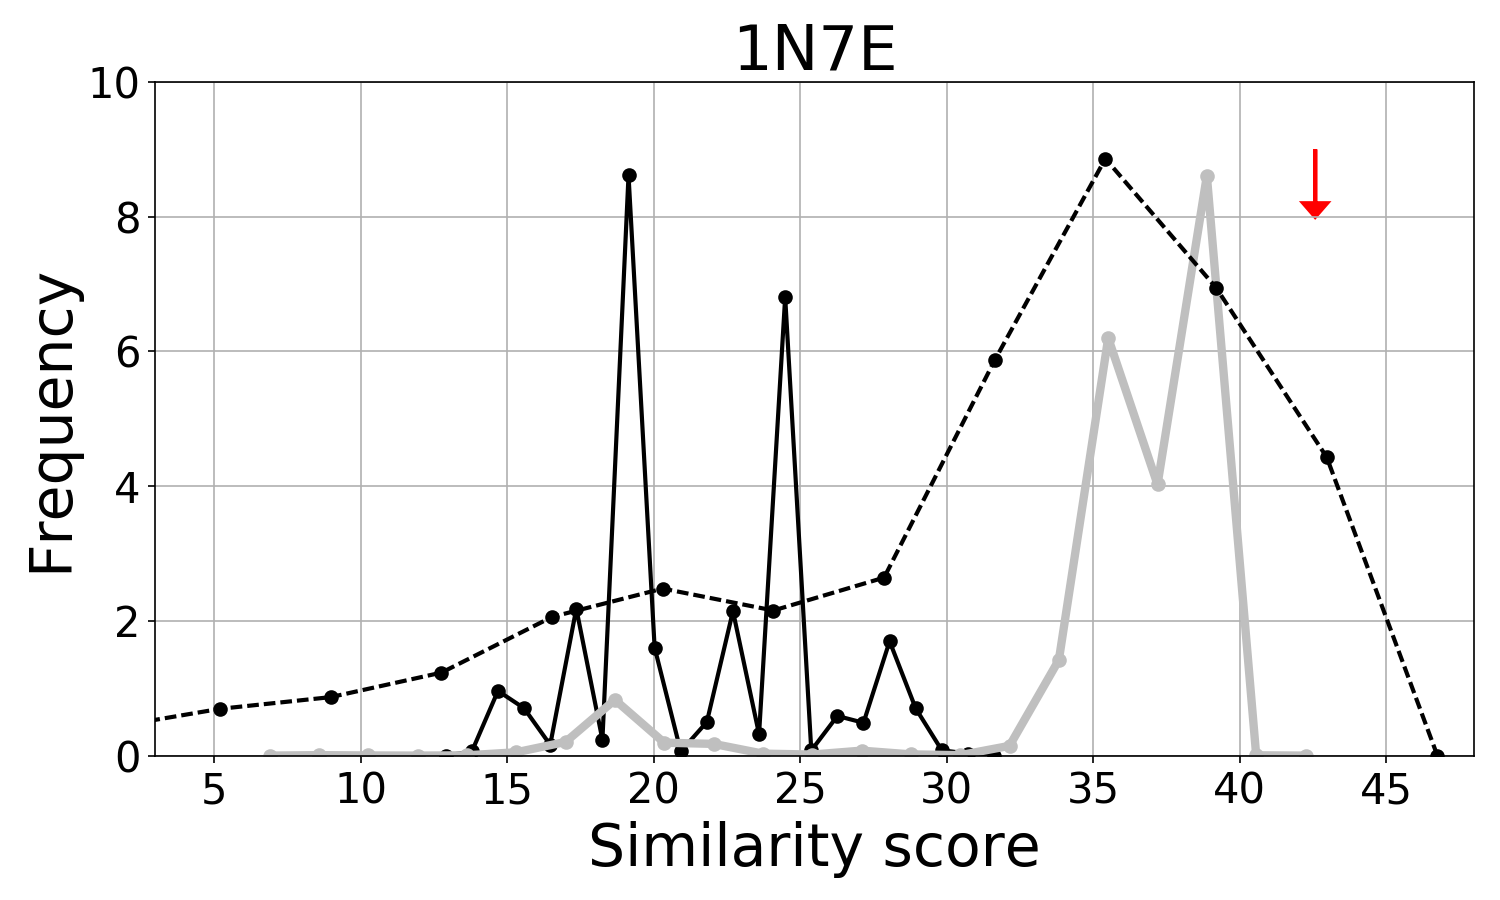
\includegraphics[width=8.4cm]{modelB6+/1N7E_simil_core.png} \\
       \includegraphics[width=8.4cm]{modelB6+/2BYG_simil_core.png} &
       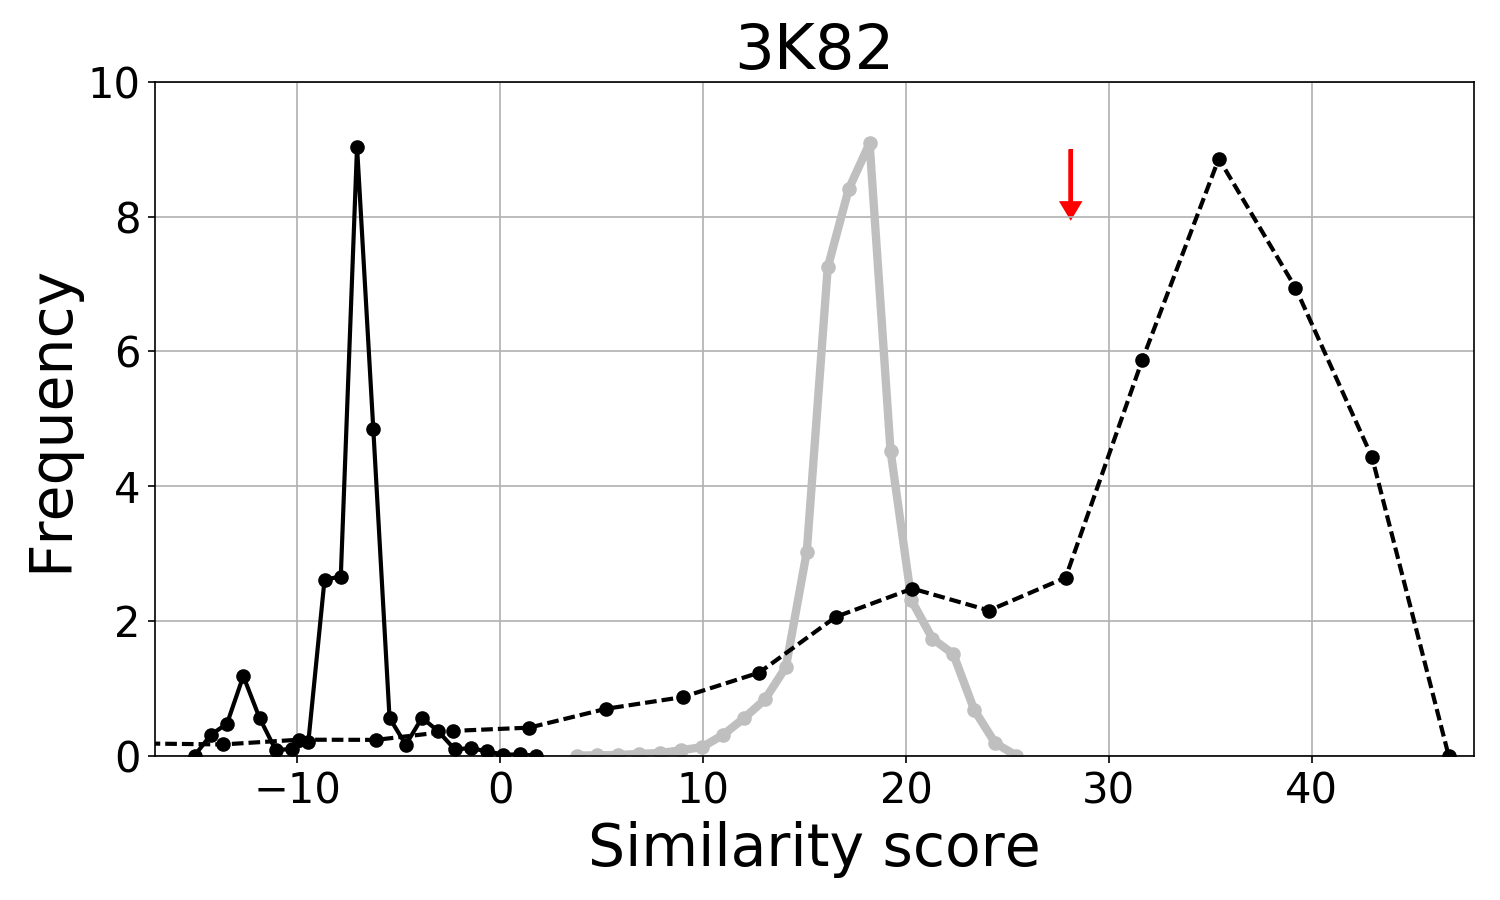
\includegraphics[width=8.4cm]{modelB6+/3K82_simil_core.png} \\
     \end{tabular}
  \caption{Similarité des séquences des 6 protéines produites par proteus modèle NEA et Rosetta à l'alignement Pfam RP55, sur les positions du cœur hydrophobe.}
\label{fig:similNEAcore}
   \end{figure}
   
   \subsection{Tests de validation croisée}
   \textbf{ Cette partie a été effectuée en commun avec Nicolas Panel, doctorant de notre laboratoire. Les détails sont publiés dans \cite{mignon2017}.}
Comme premier test de validation croisée, nous appliquons nos énergies de référence aux deux domaines de notre sous-ensemble $\mathcal(S_2)$, qui ne font pas partie du sous-ensemble utilisé dans la partie optimisation, voir \ref{subsection:freqaa}. Ainsi, nous générons des séquences Tiam1 et Cask qui sont alors soumisses aux tests Superfamily et aux calculs de similarité. La performance de Tiam1 sur la superfamille ,84,6\%, est un peu en dessous de celles obtenues sur des protéines de $\mathcal(S_1)$. Le score de Tiam1 pour la reconnaissance de la famille est à 76,6\%. Les scores de Cask sont du même ordre que ceux de nos 6 premières protéines avec 100\% de reconnaissance pour la famille et la superfamille, avec des E-values comparables.

Comme validation croisée supplémentaire, les énergies de références ont été optimisées par Nicolas Panel, en utilisant notre sous-ensemble $\mathcal(S_2)$ comme ensemble alternatif de domaines PDZ, et la troisième méthode d'optimisation, voir \ref{eq:log}. Nous générons alors, avec ce modèle, des séquences pour Syntenin et DLG2.
Encore une fois, les scores sont proches de ceux obtenus avec le modèle optimisé sur $\mathcal(S_1)$. Les reconnaissances sont à 100\% et les E-values montent de $4.01$ $10^{-4}$  à $1.3$ $10^{-2}$  avec Syntenin pour la superfamille et de $3.82$ $10^{-10}$  à $8.0$ $10^{-9}$ pour DLG2.

Les histogrammes des scores de similarité Blosum montrent que les scores globaux pour Tiam1 et Cask sont très semblables pour les deux modèles. Pour DLG2 et Syntenine, nous calculons également les scores de similarité en utilisant les deux modèles. Les scores de similarité avec le modèle $S_2$  sont légèrement plus faibles qu'avec le modèle $S_1$. Le score global a diminué d'environ 20 points pour la Synténine et environ 10 points pour DLG2. dans l'ensemble, les modèles de validation croisée ont légèrement dégradé les performances. Ainsi, pour tout domaine d'intérêt PDZ, il est préférable d'optimiser les énergies de référence spécifiquement pour ce domaine plutôt que de transférer des valeurs paramétrées en utilisant d'autres domaines PDZ. 

\section{Résultats du modèle FDB}

\subsection{optimisation du modèle de l'état déplié}

Nous optimisons maintenant les énergies de référence $E_t^r$ en utilisant la variante FDB du modèle de solvant GB , voir le paragraphe \ref{FDB}. Nous nous limitons maintenant à trois protéines: NHREF, Syntenin et DLG2. Ici, la constante diélectrique de la protéine est fixée à $4$, et un jeu de paramètres surfaciques optimisés sur ces trois protéines, voir \ref{phiaTG}. La méthode d'optimisation utilisée est la méthode parabolique voir (\ref{enumMeth}) avec 20 itérations avec la contrainte des classes de type d'acides aminés et 20 itérations sans cette contrainte,(la description est en   \label{enumMeth}). Chaque itération se fait avec 100 millions de pas. La fonction Proxy calculée sur les classes converge aux valeurs $0.06$ et $0.03$ , pour les énergies enfuies et respectivement les énergies exposées et aux valeurs $0.03$ (enfuis) et $0.02$ (exposés) pour la fonction proxy calculées sur les types. Ce qui donne pour les $E_t^r$, des fluctuations inférieures à $0,05 Kcal/mol$ sur les $5$ derniers cycles , pour tous les types, sauf pour Arg et Hip dans le cas enfui, où les variations montent à $0.1 Kcal/mol$. La population des types d'acide aminé est proche de la population sauvage. Les écarts sur les classes de types d'acide aminés dans le cas des positions enfuies sont inférieurs à 1\%  sauf pour le groupe {Asp,Glu} 1,2\%  et {Hip,Hie,Hid} 1,4\%. Dans le cas exposé, les écarts sont un peu moins bons avec 5 groupes entre 2 et 3\% , sachant que les Gly et Pro ne sont pas générés par Proteus. Les détails sont donnés dans le tableau \ref{Tab:FreqAA3}.


   \begin{table}[!htbp]
     \centering
\caption{La composition en acide aminé (\%) des séquences expérimentales et Proteus après optimisation FDB des énergies de référence. La différence entre expérimentales et Proteus sur les classes est donnée entre crochets.}
\begin{tabular}{l|cccc|cccc}
\hline
\multirow{2}{*}{Res} & \multicolumn{4}{c|}{3 protéines expérimentale}s & \multicolumn{4}{c}{FDB}\\
 & \multicolumn{2}{c}{Enfoui} & \multicolumn{2}{c|}{Exposé} & \multicolumn{2}{c}{Enfoui} & \multicolumn{2}{c}{Exposé} \\
\hline
 & type & classe & type & classe & type & classe & type & classe \\
\hline 
ALA                  & 8,7                  &  \multirow{3}{*}{16,8} & 5,5                  & \multirow{3}{*}{13,6}   &   9,6                & \multirow{2}{*}{17,1}    & 1,8 & \multirow{2}{*}{11,3} \\
CYS                  & 1,9                  &                        & 0,4                  &                         &    2,8               & \multirow{2}{*}{[-0,3]}  & 0,6 & \multirow{2}{*}{[2,3]} \\
THR                  & 6,2                  &                        & 7,7                  &                         &    4,7               &                          & 8,9 &                       \\
\hline
\multirow{2}{*}{SER} & \multirow{2}{*}{4,4} & \multirow{2}{*}{4,4}   & \multirow{2}{*}{6,7} & \multirow{2}{*}{6,7}    & \multirow{2}{*}{5,2} & 5,2                      & \multirow{2}{*}{7,9} & 7,9\\
                     &                      &                        &                      &                         &                      &  [-0,8]                  &                      & [-1,2] \\
\hline
ASP                  & 4,8                  & \multirow{2}{*}{7,4}   & 6,1                  & \multirow{2}{*}{17,1}   &   5,8                &  8,6                     & 8,1    & 20,6  \\
GLU                  & 2,6                  &                        & 11,0                 &                         &   2,8                &  [-1,2]                  & 12,5   &  [-3,5] \\
\hline
ASN                  & 3,4                  & \multirow{2}{*}{5,1}   & 6,9                  & \multirow{2}{*}{12,7}   &   4,2                &  6,0                     & 8,8 & 16,0 \\
GLN                  & 1,7                  &                        & 5,8                  &                         &   1,8                &  [-0,9]                  & 7,2 & [-3,3]    \\
\hline
HIP                  & 2,0                  & \multirow{3}{*}{2,0}   & 5,9                  & \multirow{3}{*}{5,9}    &   0,0                & \multirow{2}{*}{0,6}     & 0,4 & \multirow{2}{*}{5,0} \\
HIE                  & 0,0                  &                        & 0,0                  &                         &   0,5                & \multirow{2}{*}{[1,4]}   & 2,7 & \multirow{2}{*}{[0,9]}  \\
HID                  & 0.0                  &                        & 0.0                  &                         &   0.1                &                          & 1.9 & \\
\hline
ILE                  & 12,4                 & \multirow{3}{*}{50,3}  & 4,1                  & \multirow{3}{*}{14,0}   &   11,2               & \multirow{2}{*}{49,4}    & 0,6 & \multirow{2}{*}{12,5} \\
VAL                  & 21,1                 &                        & 5,1                  &                         &   21,2               & \multirow{2}{*}{[0,9]}   & 5,2 & \multirow{2}{*}{[1,5]}  \\
LEU                  & 16,8                 &                        & 4,8                  &                         &   17,0               &                          & 6,7 & \\
\hline
\multirow{2}{*}{MET} & \multirow{2}{*}{1.3} & \multirow{2}{*}{1,3}   & \multirow{2}{*}{1,8} & \multirow{2}{*}{1,8}    & \multirow{2}{*}{1,0} & 1,0                      & \multirow{2}{*}{2,2}  & 2,2\\
                     &                      &                        &                      &                         &                      & [0,3]                    &                       & [-0,4] \\
\hline
\multirow{2}{*}{LYS} & \multirow{2}{*}{3,4} & \multirow{2}{*}{3,4}   & \multirow{2}{*}{10,8} & \multirow{2}{*}{10,8}  & \multirow{2}{*}{4,2} & 4,2                    & \multirow{2}{*}{12,4} & 12,4  \\
                     &                      &                        &                       &                        &                       &  [-0,8]                  &                       & [-1,6] \\
\hline
\multirow{2}{*}{ARG} & \multirow{2}{*}{1,1} & \multirow{2}{*}{1,1}   & \multirow{2}{*}{9,8}  & \multirow{2}{*}{9,8}   & \multirow{2}{*}{1,8} & 1,8                      & \multirow{2}{*}{11,8} & 11,8    \\
                     &                      &                        &                      &                         &                      & [-0,7]                    &                      & [-2,0]   \\
\hline
PHE                  & 4,6                  & \multirow{2}{*}{4,6}   & 2,4                  & \multirow{2}{*}{2,5}    &  3,9                 & 3,9                      & 0,0 & 0,0 \\
TRP                  & 0,0                  &                        & 0,1                  &                         &  0,0                 & [0,7]                    & 0,0 & [2,5]               \\
\hline
TYR                  & \multirow{2}{*}{2,4} & \multirow{2}{*}{2,4}  & \multirow{2}{*}{1,2}  &   \multirow{2}{*}{1,2}  &  \multirow{2}{*}{2,0} & 2,0                     & \multirow{2}{*}{0,0}  & 0,0   \\
                     &                      &                        &                      &                         &                       & [0,4]                   &                      & [1,2]  \\
\hline
GLY                  & 1,0                  & \multirow{2}{*}{1,1}   & 1,9                  & \multirow{2}{*}{3,7}    &   0,0                &  0,0                     & 0,0 & 0,0 \\
PRO                  & 0,1                  &                        & 1,8                  &                         &   0,0                &  [1,1]                   & 0,0 & [3,7]\\
\hline

\end{tabular}
\label{tab:RefEner6}      
\end{table}


Pour pouvoir évaluer l'apport de l'optimisation FDB dans notre modèle, nous optimisons également les $E_t^r$ pour nos trois protéines avec le modèle NEA et la constante diélectrique de la protéine à $4$. La même méthode d'optimisation est utilisée.  Dans ces conditions,les $E_t^r$ se stabilisent à $0.05$ pour tous les types enfuis ou exposés. Ces 4 jeux d'énergies sont donnés dans le tableau \ref{tab:RefEner3prot}. Ainsi nous avons deux modèles qui ne different plus que par la variante GB utilisée.


    \begin{table}[!htbp]
      \centering
      \caption{Les énergies de référence obtenues avec l'optimisation sur 3 protéines. La constante diélectrique est fixé à 4.}
      \begin{tabular}{ccc|cc}

        \toprule
        \multirow{2}{*}{acides aminés}  & \multicolumn{2}{c|}{NEA} & \multicolumn{2}{c}{FDB} \\
        \cmidrule{2-5}
         & Pos. Enf. & Pos Exp. & Pos. Enf. & Pos Exp. \\
        \cmidrule{1-5}

        ALA &   0.00     &  0,00    &   0,00  &   0,00       \\
        CYS &  -0,89     &  -2,57   &  -1,06  &   -1,64      \\
        THR &  -5,31     &  -8 075  &  -4,84  &   -6,68      \\
        SER &  -5,55     &  -6,55   &  -4,45  &   -5,24      \\
        ASP &  -17,26    &  -22,06  &  -14,56 &   -18,82     \\
        GLU &  -16,12    &  -20,68  &  -14,52 &   -18,21     \\
        ASN &  -16,38    &  -20,41  &  -14,02 &   -17,80     \\
        GLN &  -14,00    &  -18,41  &  -13,14 &   -16,61     \\
        HID &   11.21    &  6.95    &  10.85  &   8.13       \\
        HIE &   10,63    &  6,15    &  10,41  &   7,37       \\
        HIP &   15,17    &  10,72   &  12,86  &   10,98      \\
        ARG &  -53,40    &  -57,36  &  -51,37 &   -54,76     \\
        LYS &  -8,20     &  -12,34  &  -8,24  &   -11,35     \\
        ILE &   6,76     &  3,44    &  5,50   &   3,06       \\
        VAL &   0,43     &  -2,19   &  -0,05  &   -1,66      \\
        LEU &   0,52     &  -3,72   &  0,00   &   -2,94      \\
        MET &  -1,61     &  -3,21   &  -2,85  &   -3,09      \\
        PHE &   1.86     &  -2,68   &  0,17   &   -3,18      \\
        TRP &  -0,23     &  -7,67   &  -1,94  &   -5,53      \\
        TYR &  -5,10     &  -10,90  &  -5,91  &   -10,14     \\

        \bottomrule

      \end{tabular}      

\label{tab:RefEner3prot}      
    \end{table}

    
\subsection{Tests de reconnaissance de famille}
À présent, nous générons des séquences pour chaque protéine et pour chacun des jeux des $E_t^r$ FDB et NEA. Le protocole pour Proteus est identique à celui utilisé voir de la section \ref{sectionNEA},la constante diélectrique de la protéine étant maintenant de $4$. Ici encore, les 10 000 séquences de meilleures énergies parmi celles échantillonnées par les répliques REMC sont retenues pour l'analyse. Les résultats Superfamily sont présentés au tableau \ref{tab:superfamily3prot}. Pour le FDB, la reconnaissance des familles et des superfamilles est de 100\% pour les 3 protéines tout comme Rosetta. En termes de E-value, Proteus FDB fait jeu égal avec Rosetta, avec des valeurs pour la superfamille allant de $2.85$ $10^{-6}$ jusqu'à $8.54$ $10^{-14}$ pour Proteus et allant de $1.3$ $10^{-9}$ à $1.3$ $10^{-13}$ pour Rosetta et des valeurs très proches pour la famille. Pour le NEA, les résultats sont corrects pour la reconnaissance avec 98\% pour les trois protéines, mais nettement moins bons pour les E-values de la superfamille. 


\begin{table}[h]
  \raggedleft{}
  
  \begin{tabular}{ccccccc}
    
    \toprule
    Model &Protein & Match/seq & Superfamily & Superfamily & Family & Family \\
            & size      & E-value      & success     & E-value & success\\
    \cmidrule{1-7}
    Proteus                   & NHREF     & 80/91  &  8.54 $10^{-14}$  & 10000  & 8.94 $10^{-3}$ & 10000 \\
    FDB                       & Syntenin  & 70/82  &  2.85 $10^{-6}$   & 10000  & 2.69 $10^{-3}$ & 10000 \\
    epsilon=4                 & DLG2      & 88/97  &  3.26 $10^{-12}$  & 10000  & 1.96 $10^{-3}$ & 10000 \\
    \cmidrule{1-7}
    \multirow{3}{*}{Rosetta}  & NHREF     & 79/91  &  1.3 $10^{-13}$ & 10000    & 2.2 $10^{-3}$ & 10000 \\
                              & Syntenin  & 76/82  &  7.3 $10^{-13}$ & 10000    & 1.8 $10^{-3}$ & 10000 \\
                              & DLG2      & 86/97  &  1,3 $10^{-9}$  & 10 000    & 9,6 $10^{-4}$ & 10 000 \\    
    \cmidrule{1-7}
    Proteus                   & NHREF     & 62/91 &   3,22 $10^{-3}$  & 9857    & 1,00 $10^{-2}$ & 9857 \\
    NEA                       & Syntenin  & 70/82 &   2.83 $10^{-3}$  & 9879    & 3,62 $10^{-3}$ & 9879 \\
    epsilon=4                 & DLG2      & 83/97 &   1,66 $10^{-3}$  & 9876    & 3,18 $10^{-3}$ & 9876 \\ 
    \bottomrule        
  \end{tabular}   
  \caption{Résultats Superfamily pour les séquences Proteus avec le modèle FDB (énergies de références optimisées sur 20 cycles selon les classes + 20 cycles selon les types).}   
  \label{tab:superfamily3prot}       
\end{table}


\subsection{Scores de similarité Blosum}
Les scores de similarité Blosum40 sont calculés entre les séquences conçues par informatique et les séquences Pfam. Nous calculons ces similarités pour les séquences proteus FDB, proteus NEA et Rosetta, sur l'ensemble des positions sauf une petite partie au début et une petie partie à la fin de la séquence, parce qu'elles ne sont pas conservées dans l'alignement Pfam.
Cela représente moins de 10\% de la longueur de la séquence. Pour NHREF, l'approximation FDB améliore très nettement les scores de Proteus NEA avec un écart d'environ 50 points. Ce qui place Proteus à peu près au niveau de Rosetta. Pour Syntenin, les écarts sont plus serrés avec le FDB légèrement moins bon que le NEA, mais qu'en même proche de Rosetta. Dans le cas de DLG2,le FDB domine les séquences NEA et près de la moitié de celles produites par Rosetta. Sur les positions du cœur hydrophobe, Les résultats Proteus sont excellents, avec le plus souvent, des similarités avec Pfam compris entre 30 et 40. Le NEA et le FDB font jeu égal sur DLG2, le NEA étant au-dessus pour les deux autres. Il n'y a donc pas d'amélioration sur le cœur ce qui s'explique par le fait que ces résidus sont trop éloignés du solvant pour bénéficier de l'effet de l'approximation FDB. Les scores Rosetta pour Syntenin sont proches, mais pour les deux autres, les scores nettement plus variables et globalement moins bons. Tout cela est représenté à la figure  \ref{{graph:Simil_3prot}}.

   \begin{figure}[t]
     \centering
     \begin{tabular}{cc} 
       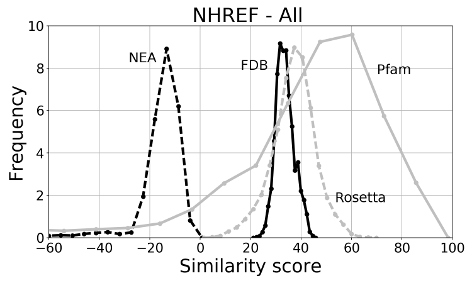
\includegraphics[width=8.4cm]{FDB/1G9O_simil_cut.png} &
       \includegraphics[width=8.4cm]{FDB/1G9O_simil_core.png} \\
       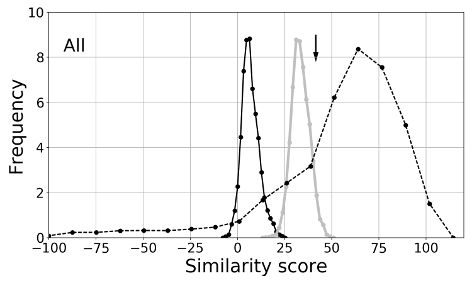
\includegraphics[width=8.4cm]{FDB/1R6J_simil_cut.png} &
       \includegraphics[width=8.4cm]{FDB/1R6J_simil_core.png} \\
       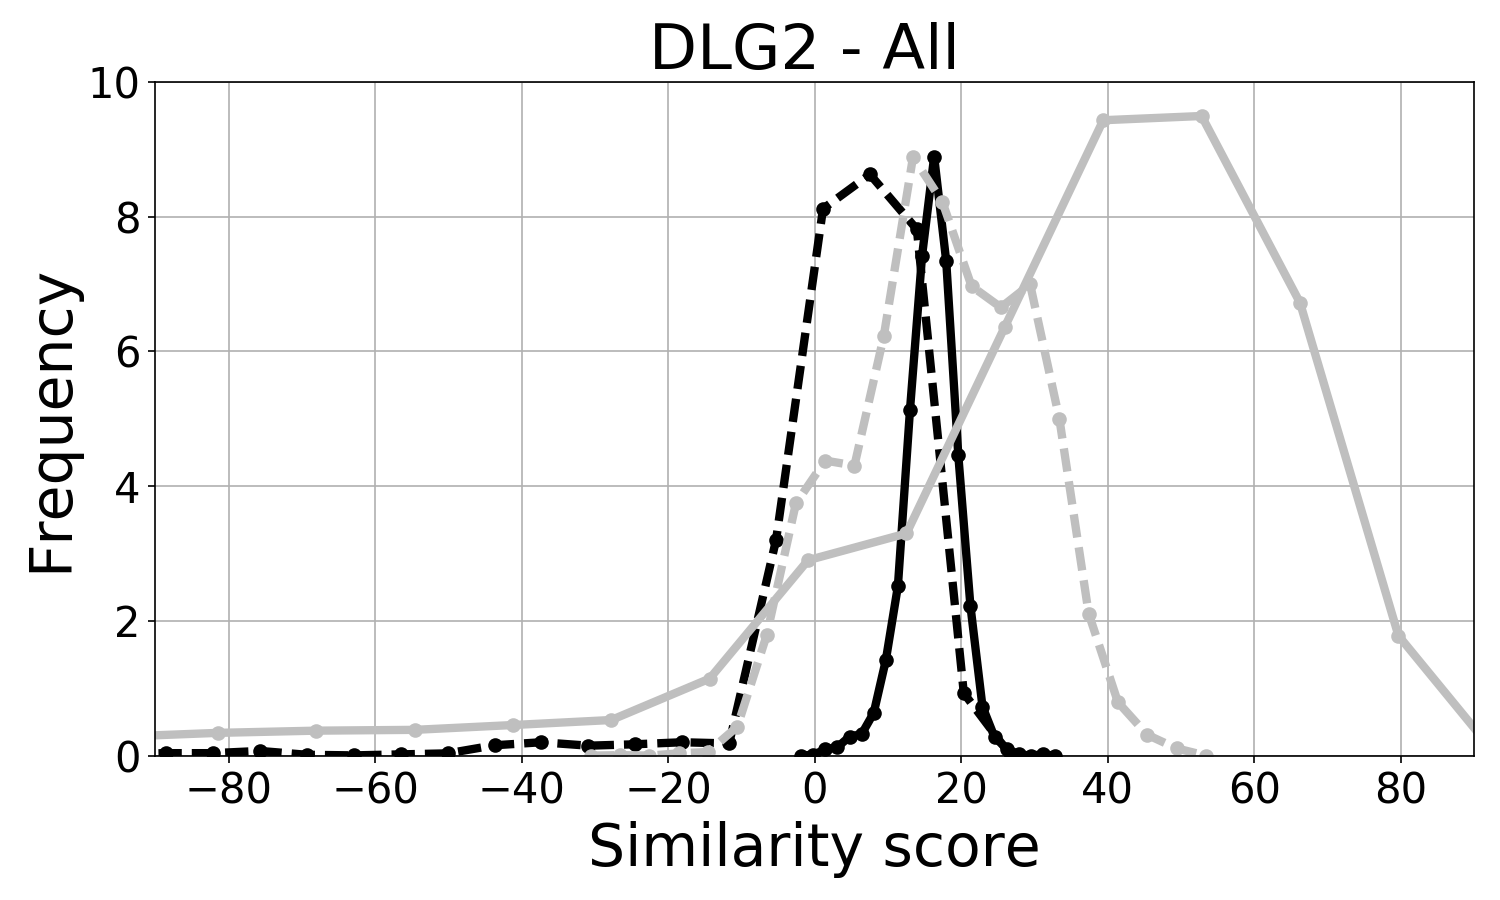
\includegraphics[width=8.4cm]{FDB/2BYG_simil_cut.png} &
       \includegraphics[width=8.4cm]{FDB/2BYG_simil_core.png} \\
     \end{tabular}
     \caption{Similarité des séquences Proteus (NEA et FDB),Rosetta , et des séquences de l'alignement Pfam RP55, sur toutes les positions à gauche  et sur les positions du cœur à droite.}

     \label{graph:Simil_3prot}
   \end{figure}

  
\subsection{Taux d'identité à la séquence native}  
  
Pour chaque protéine, nous calculons le taux d'identité des 10 000 séquences de meilleures énergies par rapport à la séquence native, ainsi que pour les 10 000 séquences Rosetta ,voir \ref{TauxID}. On considère uniquement les positions mutables sans celles aux extrémités des séquences comme expliqué au paragraphe précédent. Ce taux varie pour Proteus FDB entre 24\% et 33\% , et entre 20\% et 33\% pour la version NEA. Pour Rosetta les taux se situent entre 35 et 40\% avec un écart de 11\% pour NHREF sur le FDB et de 7\% pour les deux autres protéines. voir la table \ref{tab:IdentNEA}. Il s'avère donc que les séquences Rosetta sont nettement plus proches des séquences natives que celles de Proteus.  

\begin{table}[!htbp]
      \centering

      \begin{tabular}{cccc}

        \toprule
        Sequences & Proteus FDB & Proteus NEA & Rosetta \\
        \cmidrule{1-4}
        NHREF     & 24 & 20 & 35 \\
        Syntenin  & 31 & 33 & 38 \\
        DLG2      & 33 & 31 & 40 \\
        \bottomrule

      \end{tabular}      
      \caption{Pourcentage d'identité moyen à la séquence native}
\label{tab:IdentNEA}      
    \end{table}

\subsection{Logos des séquences obtenues}

Finalement, nous montrons les séquences obtenues. Elles sont représentées sous forme de logos à la figure \ref{logo:corePDZ} pour les positions du cœur hydrophobe, et la figure \ref{logo:} pour les positions exposées. L'accord avec les séquences naturelles sur les positions du cœur est très bon et l'accord sur les positions exposées est nettement moins bon. Mais au regard de la diversité des types aux positions exposées dans les séquences naturelles de Pfam le consensus entre les séquences naturelles est lui-même quasi inexistant.

   \begin{figure}[t]
     \scalebox{0.8}{
       \begin{tabular}{c}
         \includegraphics[width=18cm]{logos/core.png} \\
       \end{tabular}
     }
     \caption{Les séquences conçues par Proteus et les séquences naturelles représentées sous forme de logo pour les positions du cœur hydrophobe}
\label{logo:corePDZ}
   \end{figure}

   \begin{figure}[t]
     \scalebox{0.8}{
       \begin{tabular}{c}
         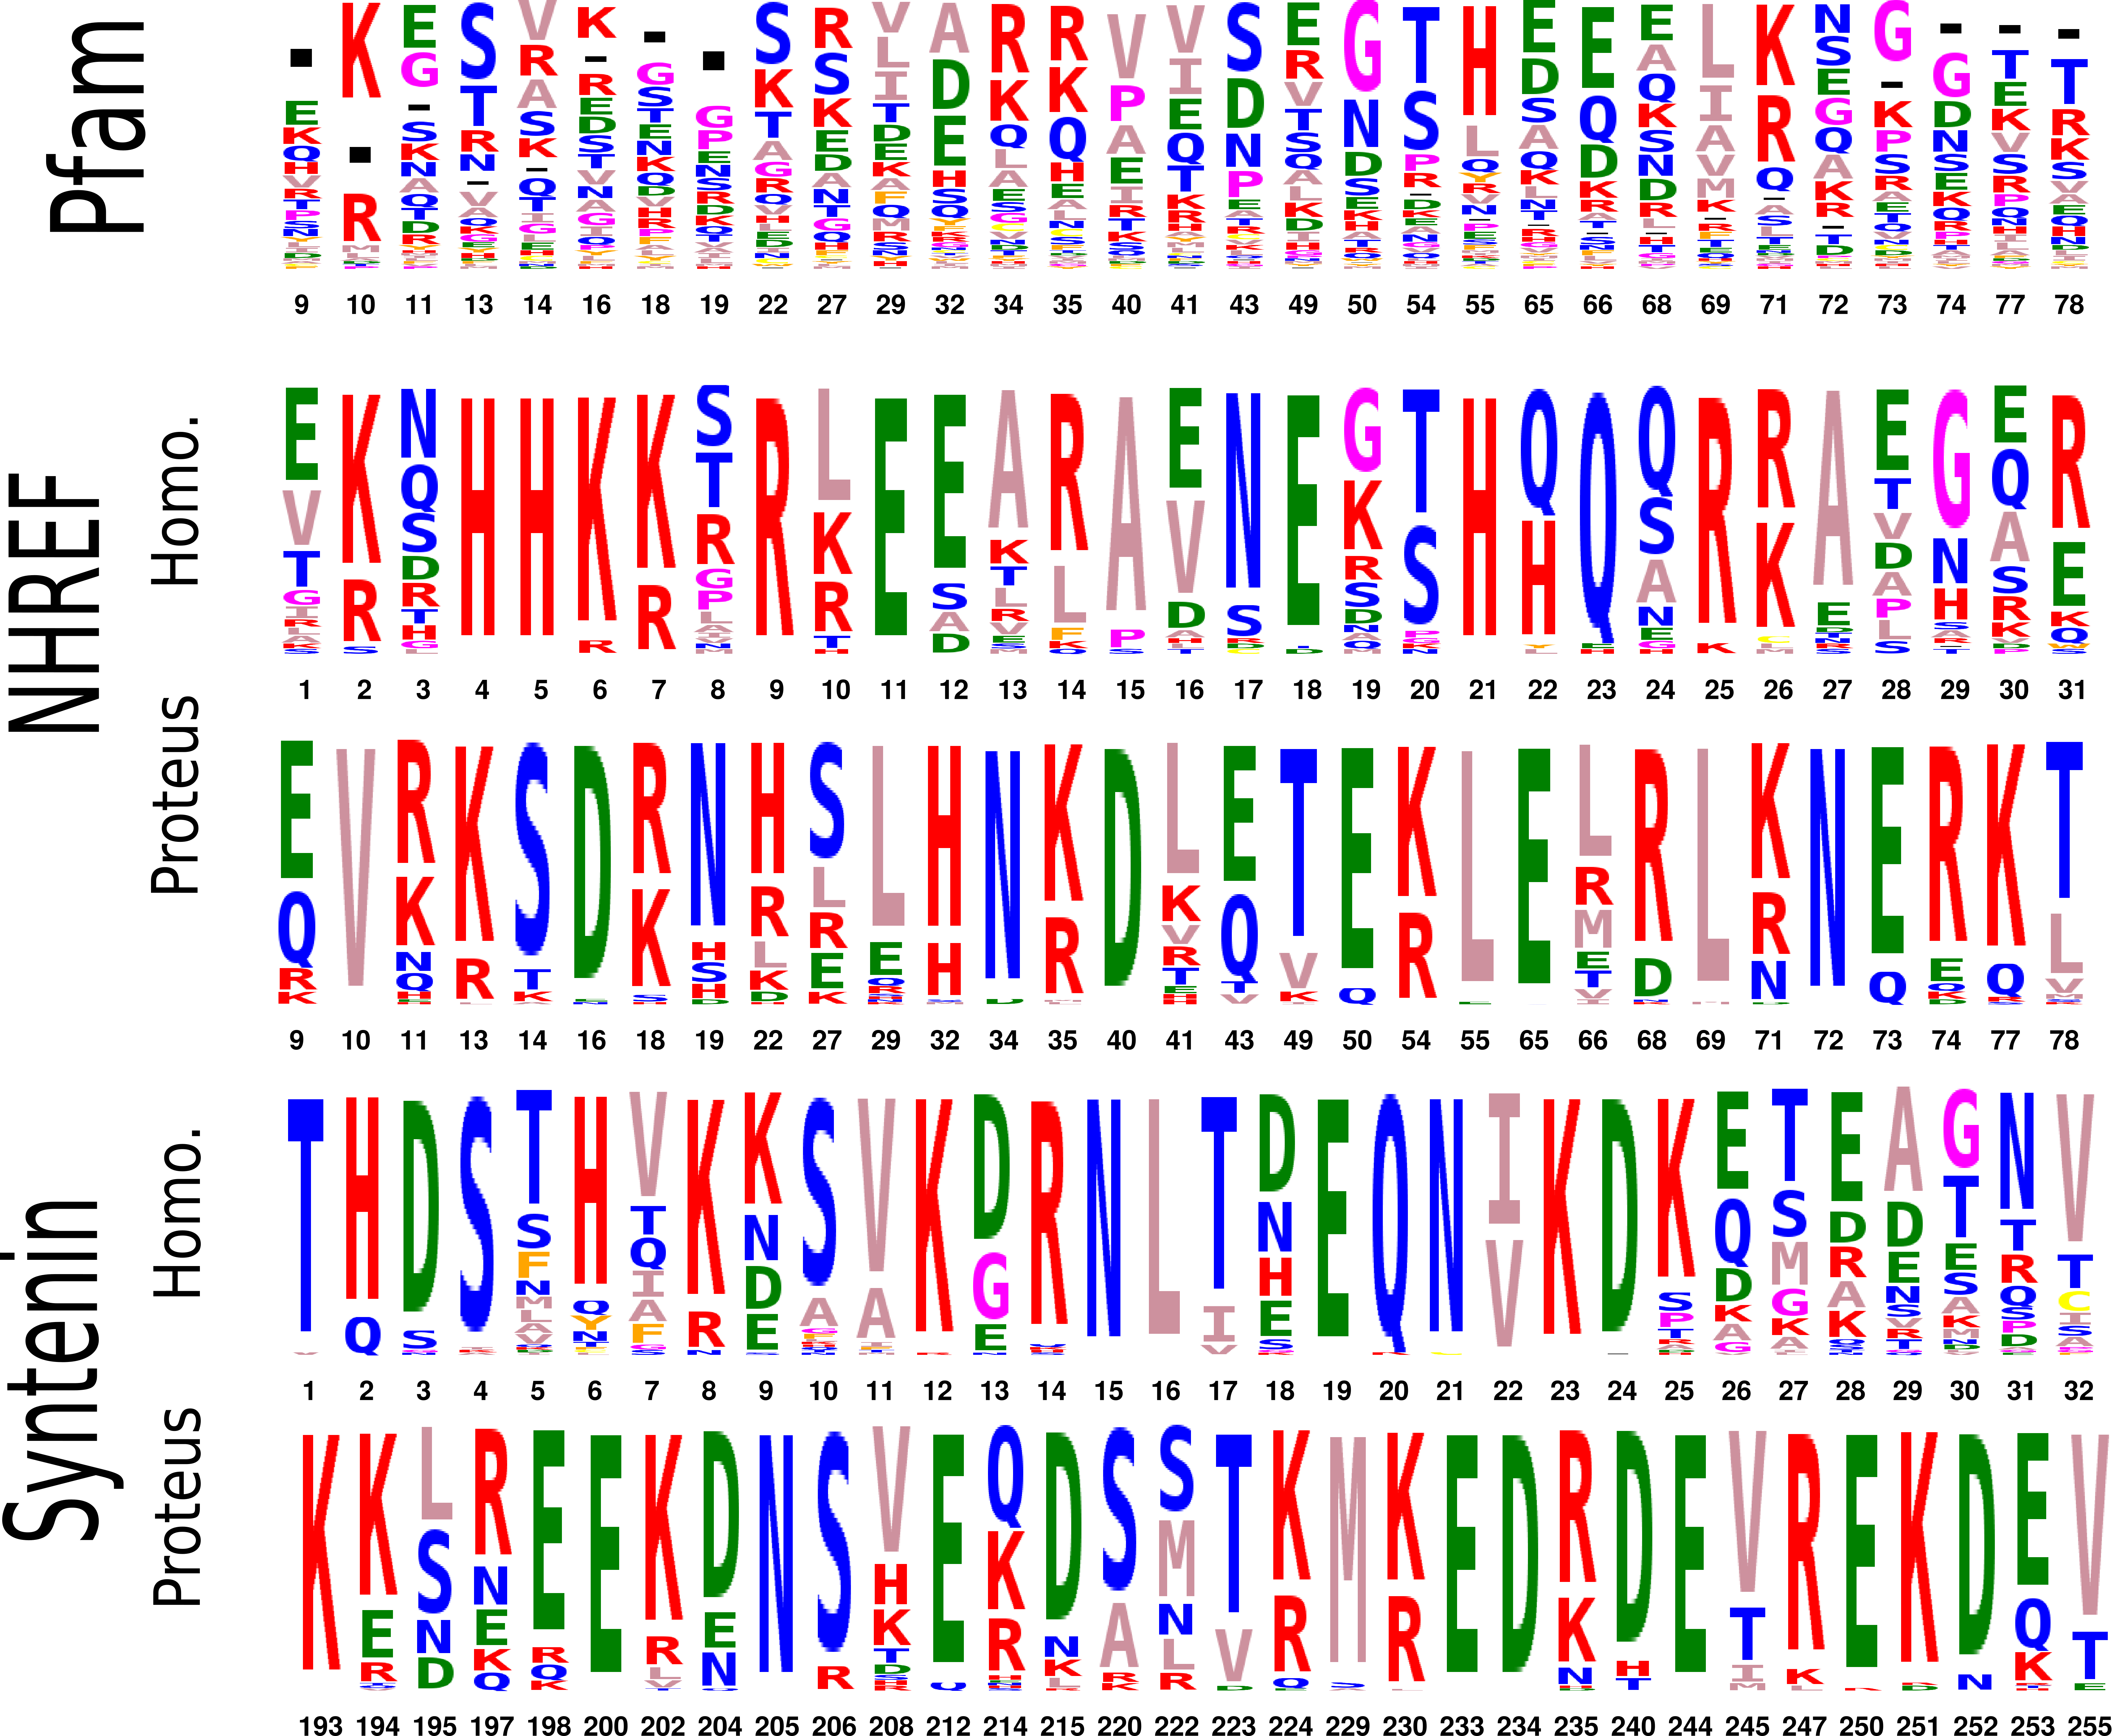
\includegraphics[width=18cm]{logos/exposed.png} \\
       \end{tabular}
     }
     \caption{Les séquences conçues par Proteus et les séquences naturelles représentées sous forme de logo pour les positions du cœur hydrophobe}
\label{logo:corePDZ}
   \end{figure}


    
\section{Application: Croissance du noyau hydrophobe}
Comme application de nos modèles optimisés, nous examinons une possibilité de \og design\fg du cœur hydrophobe des domaines PDZ. Deux de nos domaine PDZ ,Tiam1 et Cask, sont soumis à une simulation REMC avec une succession de fonctions énergétiques biaisées qui favorisent progressivement les résidus hydrophobes. La première simulation comprend un terme d'énergie avec un biais $\delta =0,4 kcal/mol$ par position, qui pénalise les types d'acides aminés hydrophobes (I,L,M,V,A,W,F et Y). Le biais augmente alors graduellement, et passe par les valeurs intermédiaires $\delta =0,2 $,$\delta =0$ et  $\delta = -0,2 kcal/mol$. La dernière simulation comprend un terme d'énergie de biais $\delta = -0.4 kcal/mol$ (par position) qui favorise les types hydrophobes. En diminuant progressivement la valeur du biais d'énergie $\delta$, nous \og titrons \fg efficacement les résidus hydrophobes.

      \caption{\small Séquences Tiam1 obtenues avec un delta des énergies de références à -0,4,-0,2,0,0.2 et 0,4 et la structure native.Les hydrophobes pour des deltas de -0,4,-0,2,0,0.2 et 0,4 sont représentés par un dégradé allant du rouge foncé au vert clair, en passant par le jaune.}


    \begin{figure}[!htbp]
      \centering
      \begin{tabular}{c}
        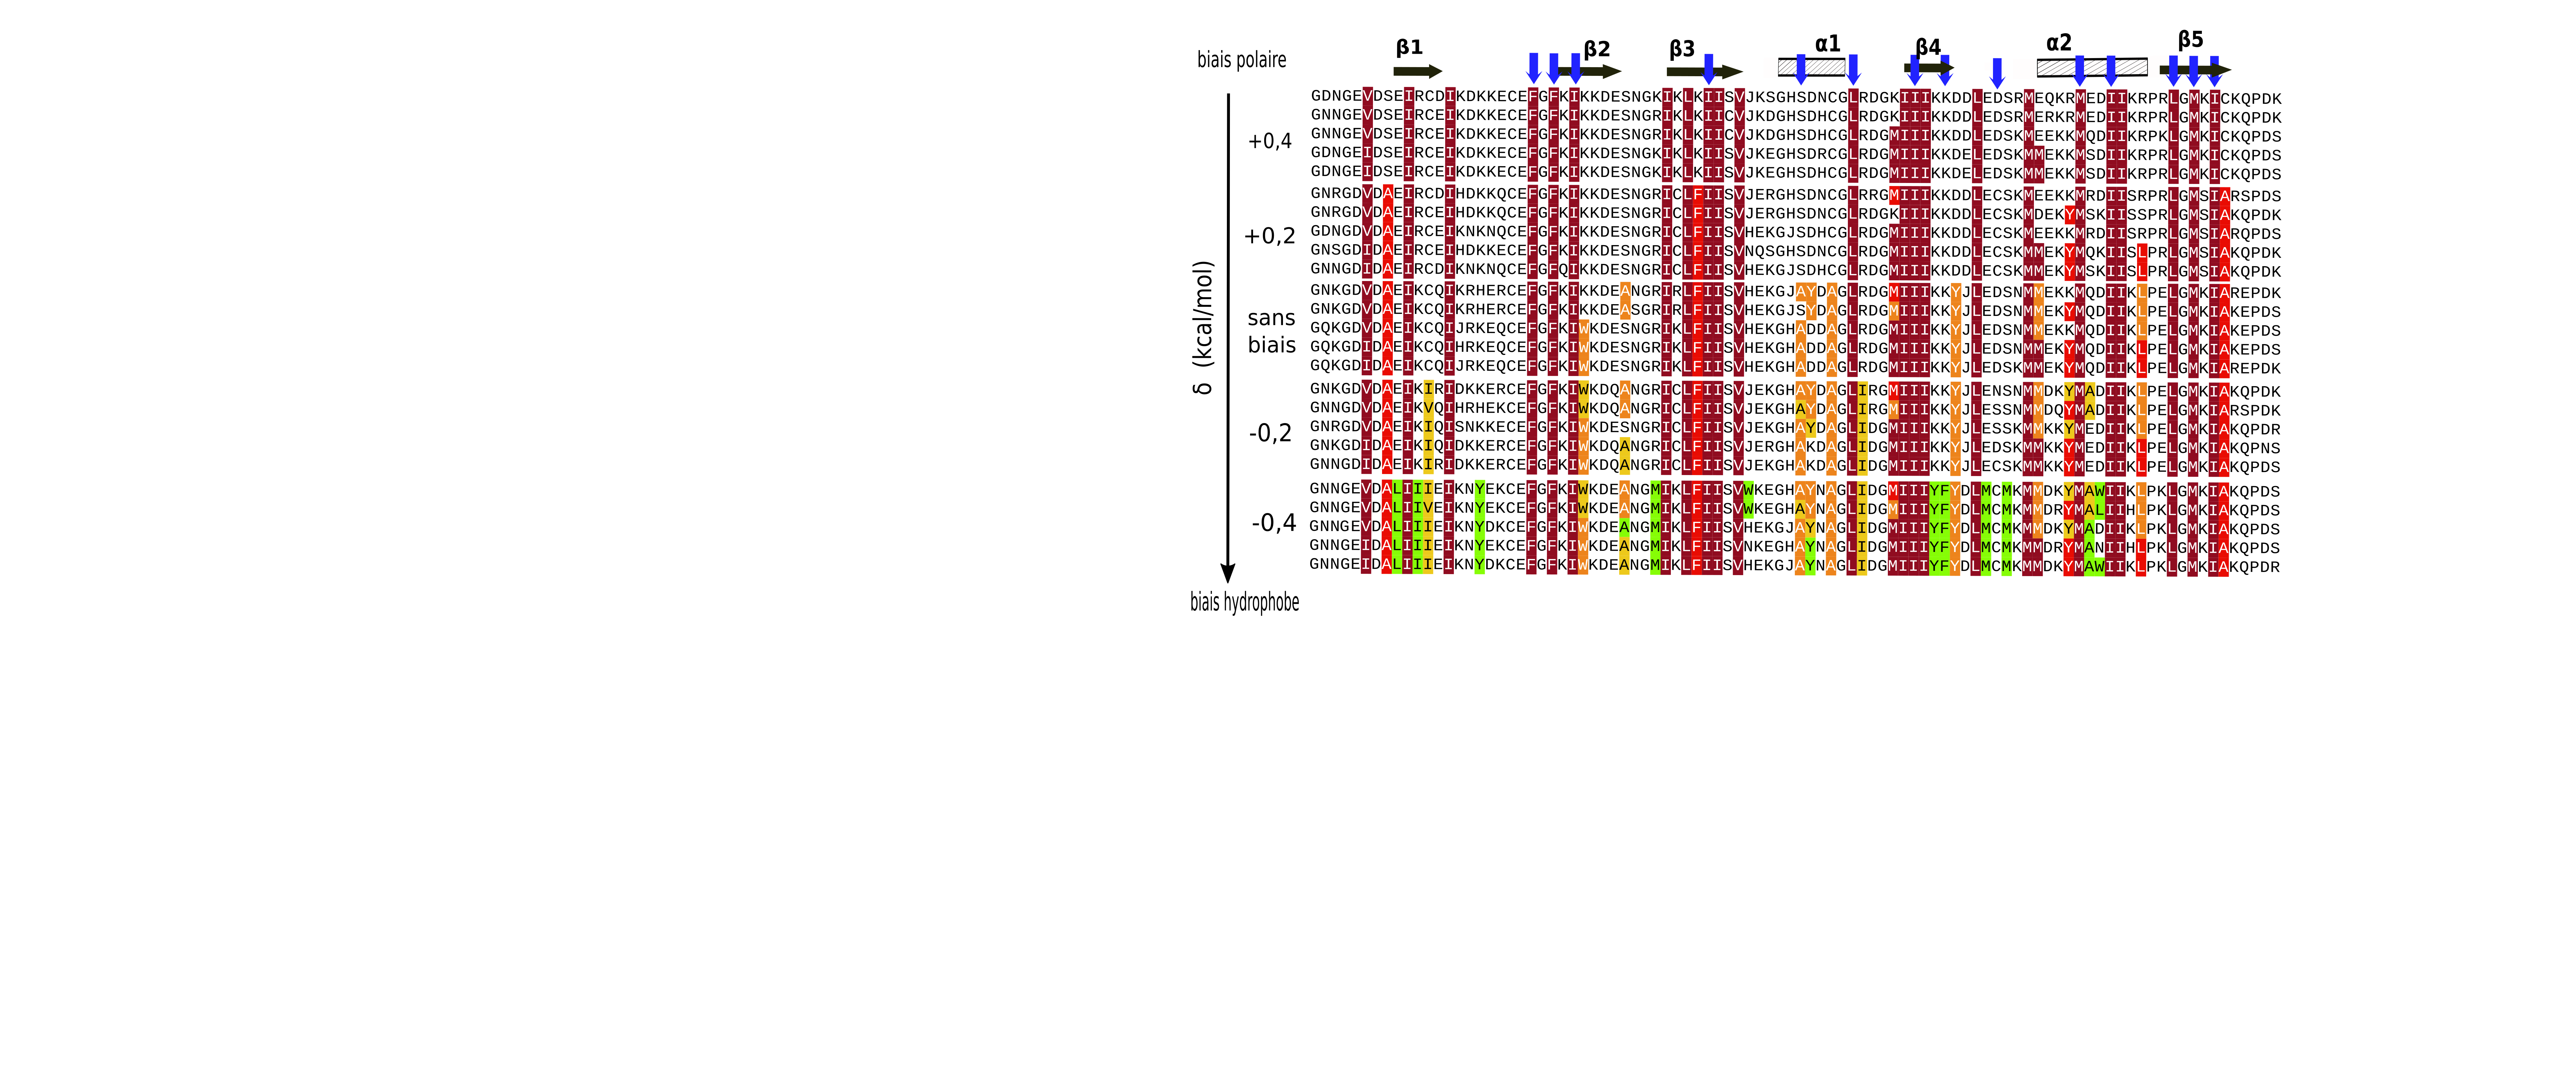
\includegraphics[width=20cm]{titration/alignTiam1.png} \\
      \end{tabular}      
      \label{titrationAlignTiam1}
            {\footnotesize Les flèches bleues indiquent les positions du cœur hydrophobe PDZ défini à partir de notre sélection de 6 domaines.Chaque groupe de séquences est une sélection à $\delta$ fixé parmi les séquences de plus faible énergie.}

    \end{figure}

\begin{landscape}
    \begin{figure}[!htbp]
      \centering
      \caption{\small Structure native Tiam1 avec les hydrophobes pour des $\delta$ de -0,4,-0,2,0,0.2 et 0,4 sont représentés par un jeu de couleurs allant du rouge foncé au vert clair, en passant par le jaune.}

      \begin{tabular}{c}
        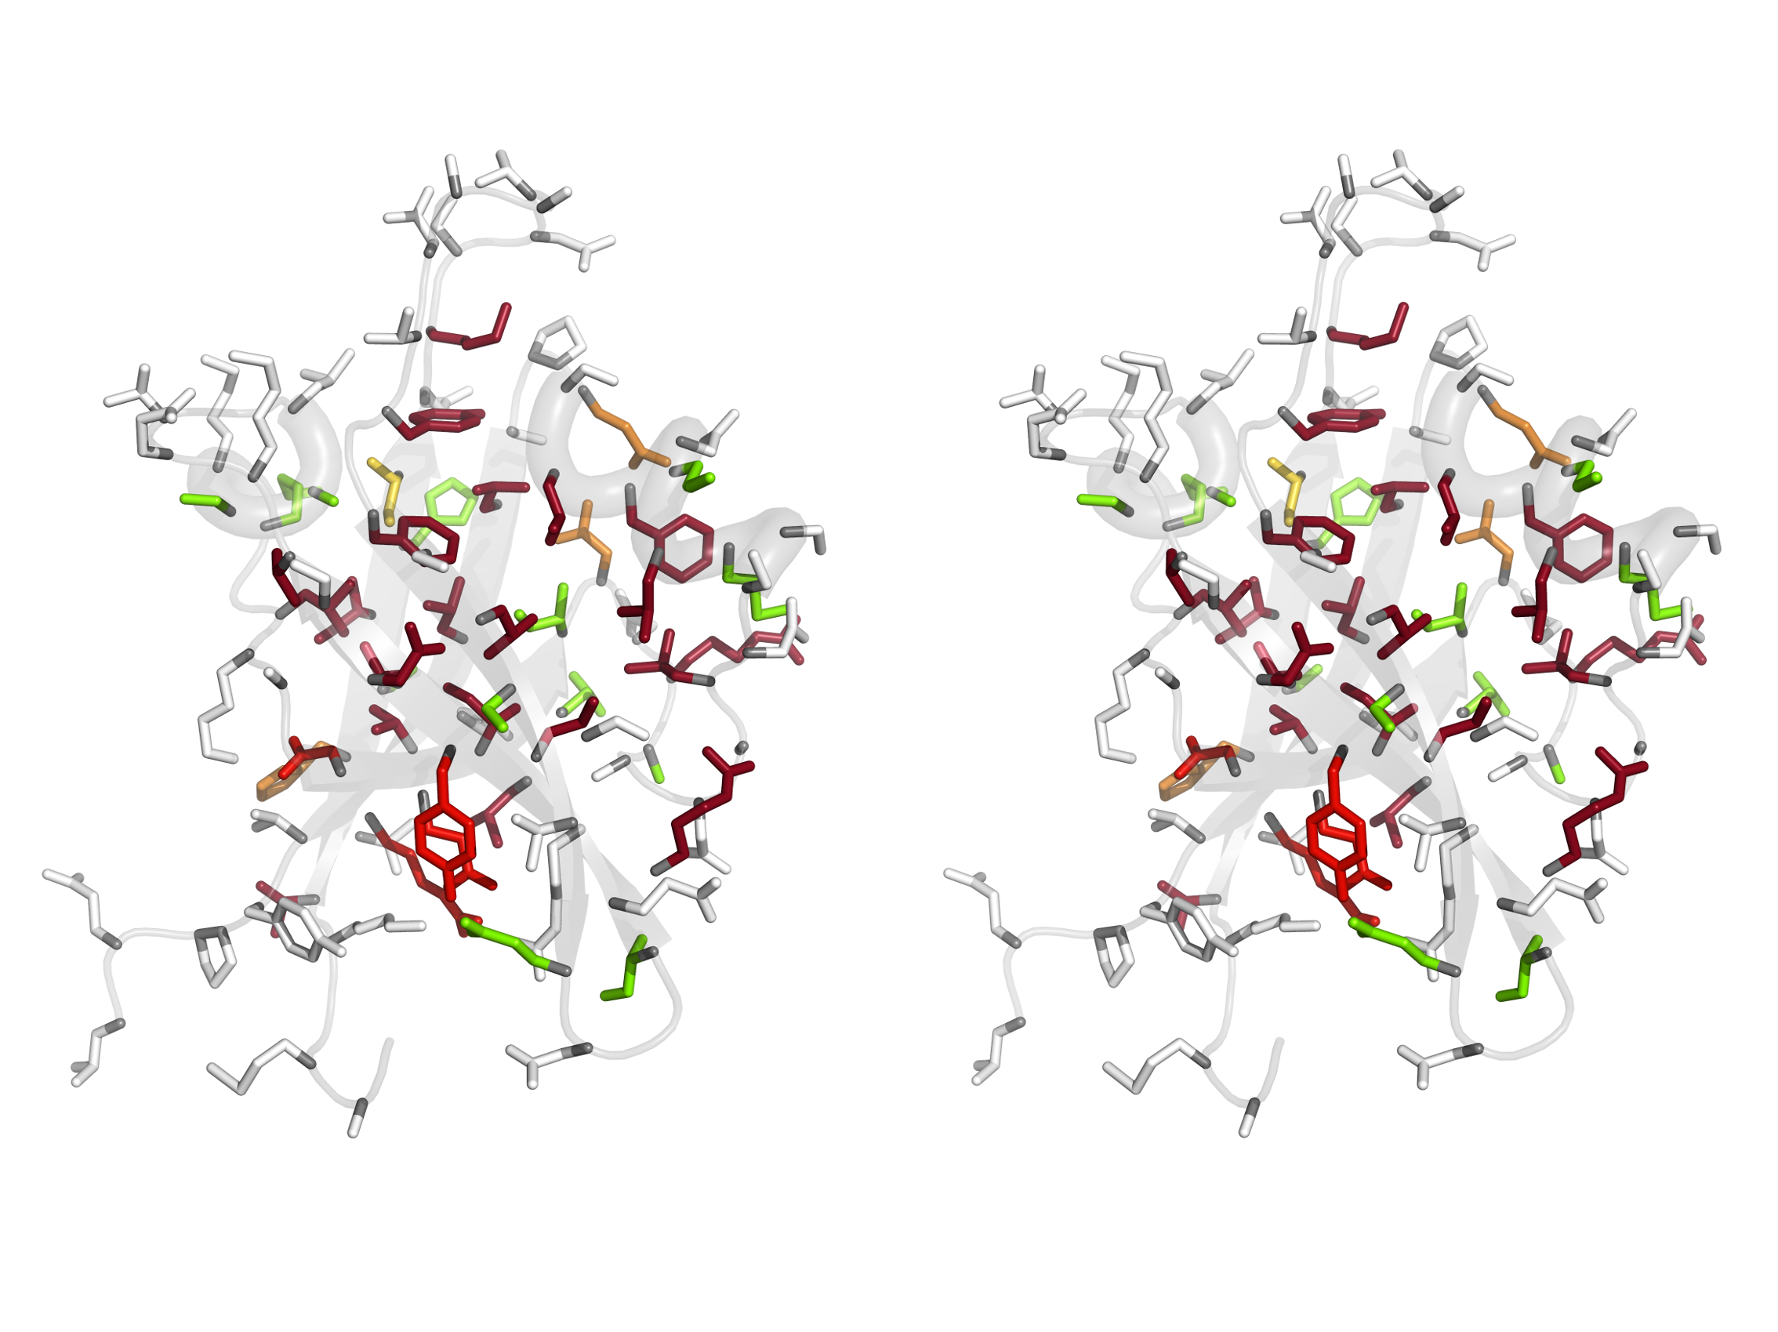
\includegraphics[width=20cm]{titration/structure_Tiam1.png} \\
      \end{tabular}
      
      \label{titrationStructTiam1}
    \end{figure}

\end{landscape}

Les résultats pour Tiam1 sont présentés à la figure \ref{titrationAlignTiam1} et à la figure \ref{titrationStructTiam1}. À la plus grande valeur de $\delta$ le cœur hydrophobe de Tiam1 est réduit à environ 10 positions (environ parce qu'il s'agit d'une sélection de séquences) d'acides aminés sur 94 qui changent en un type polaire par rapport aux séquences sans biais. Les positions modifiées se situent principalement sur le bord extérieur du cœur. A la valeur intermédiaire de $\delta$ à $0,2 kcal/mol$, le cœur hydrophobe ne compte plus que 4 ou 5 changements en type polaire. À la valeur de $\delta$ la plus négative, le cœur hydrophobe devient plus grand, s'étendant vers les régions de surface , avec globalement 14 positions polaires changées en type hydrophobe. Ainsi le nombre de positions modifiées est approximativement symétrique ( environ +/- 12 changements), reflétant le biais. Environ 2 tiers des changements se produisent dans des éléments de structure secondaire. Dans l'ensemble, les propensions observées de chaque position à devenir polaire ou hydrophobe en présence d'un biais de pénalité petit ou grand d'énergie $\delta$ peuvent être considérées comme un indice de design hydrophobe. Ici, 11 des 14 positions du cœur PDZ (toute sauf les positions 884 898 et 903) sont restées hydrophobes au plus haut niveau de biais polaire, avec à peu près 13 autres positions, indiquant que ces positions ont la plus grande propension à être hydrophobe. De plus, près de 14 positions ont basculé de polaire à hydrophobe au niveau de polarisation le plus élevé, indiquant que ces positions aussi ont une certaine propension a être hydrophobe. Les résultats pour Cask sont similaires, avec 11 positions changés en polaire au plus haut biais polaire et 9 changés en hydrophobe au plus haut biais hydrophobe, voir \ref{titrationAlignCask}.

Nous introduisons alors un indice pour décrire le nombre de changements relatifs de type d'acide aminé par unité d'énergie du biais. Cet indice  $\psi_h$ est défini comme le nombre $\delta N$ de positions qui ont changées de non polaire à polaire, divisé par le produit de la variation $\delta E$ dans l'énergie de polarisation et le nombre moyen N de positions non polaires à biais nul. Nous appelons $\psi_h$ la sensibilité hydrophobe. Pour le domaine PDZ Tiam1, ce calcul donne:
$\psi_h = \frac{1}{N} \frac{\delta N}{\delta E} = 0,9$ changements par position et par kcal/mol. Pour Cask, la sensibilité hydrophobe  est  $\psi_h = 0,7$ changements par position et par kcal/mol.


\begin{figure}[!h]
  \centering
  \caption{\small Structure native Cask avec les hydrophobes pour des $\delta$ de -0,4,-0,2,0,0.2 et 0,4 sont représentés par un dégradé allant du rouge foncé au vert clair, en passant par le jaune.}

  \begin{tabular}{c}
    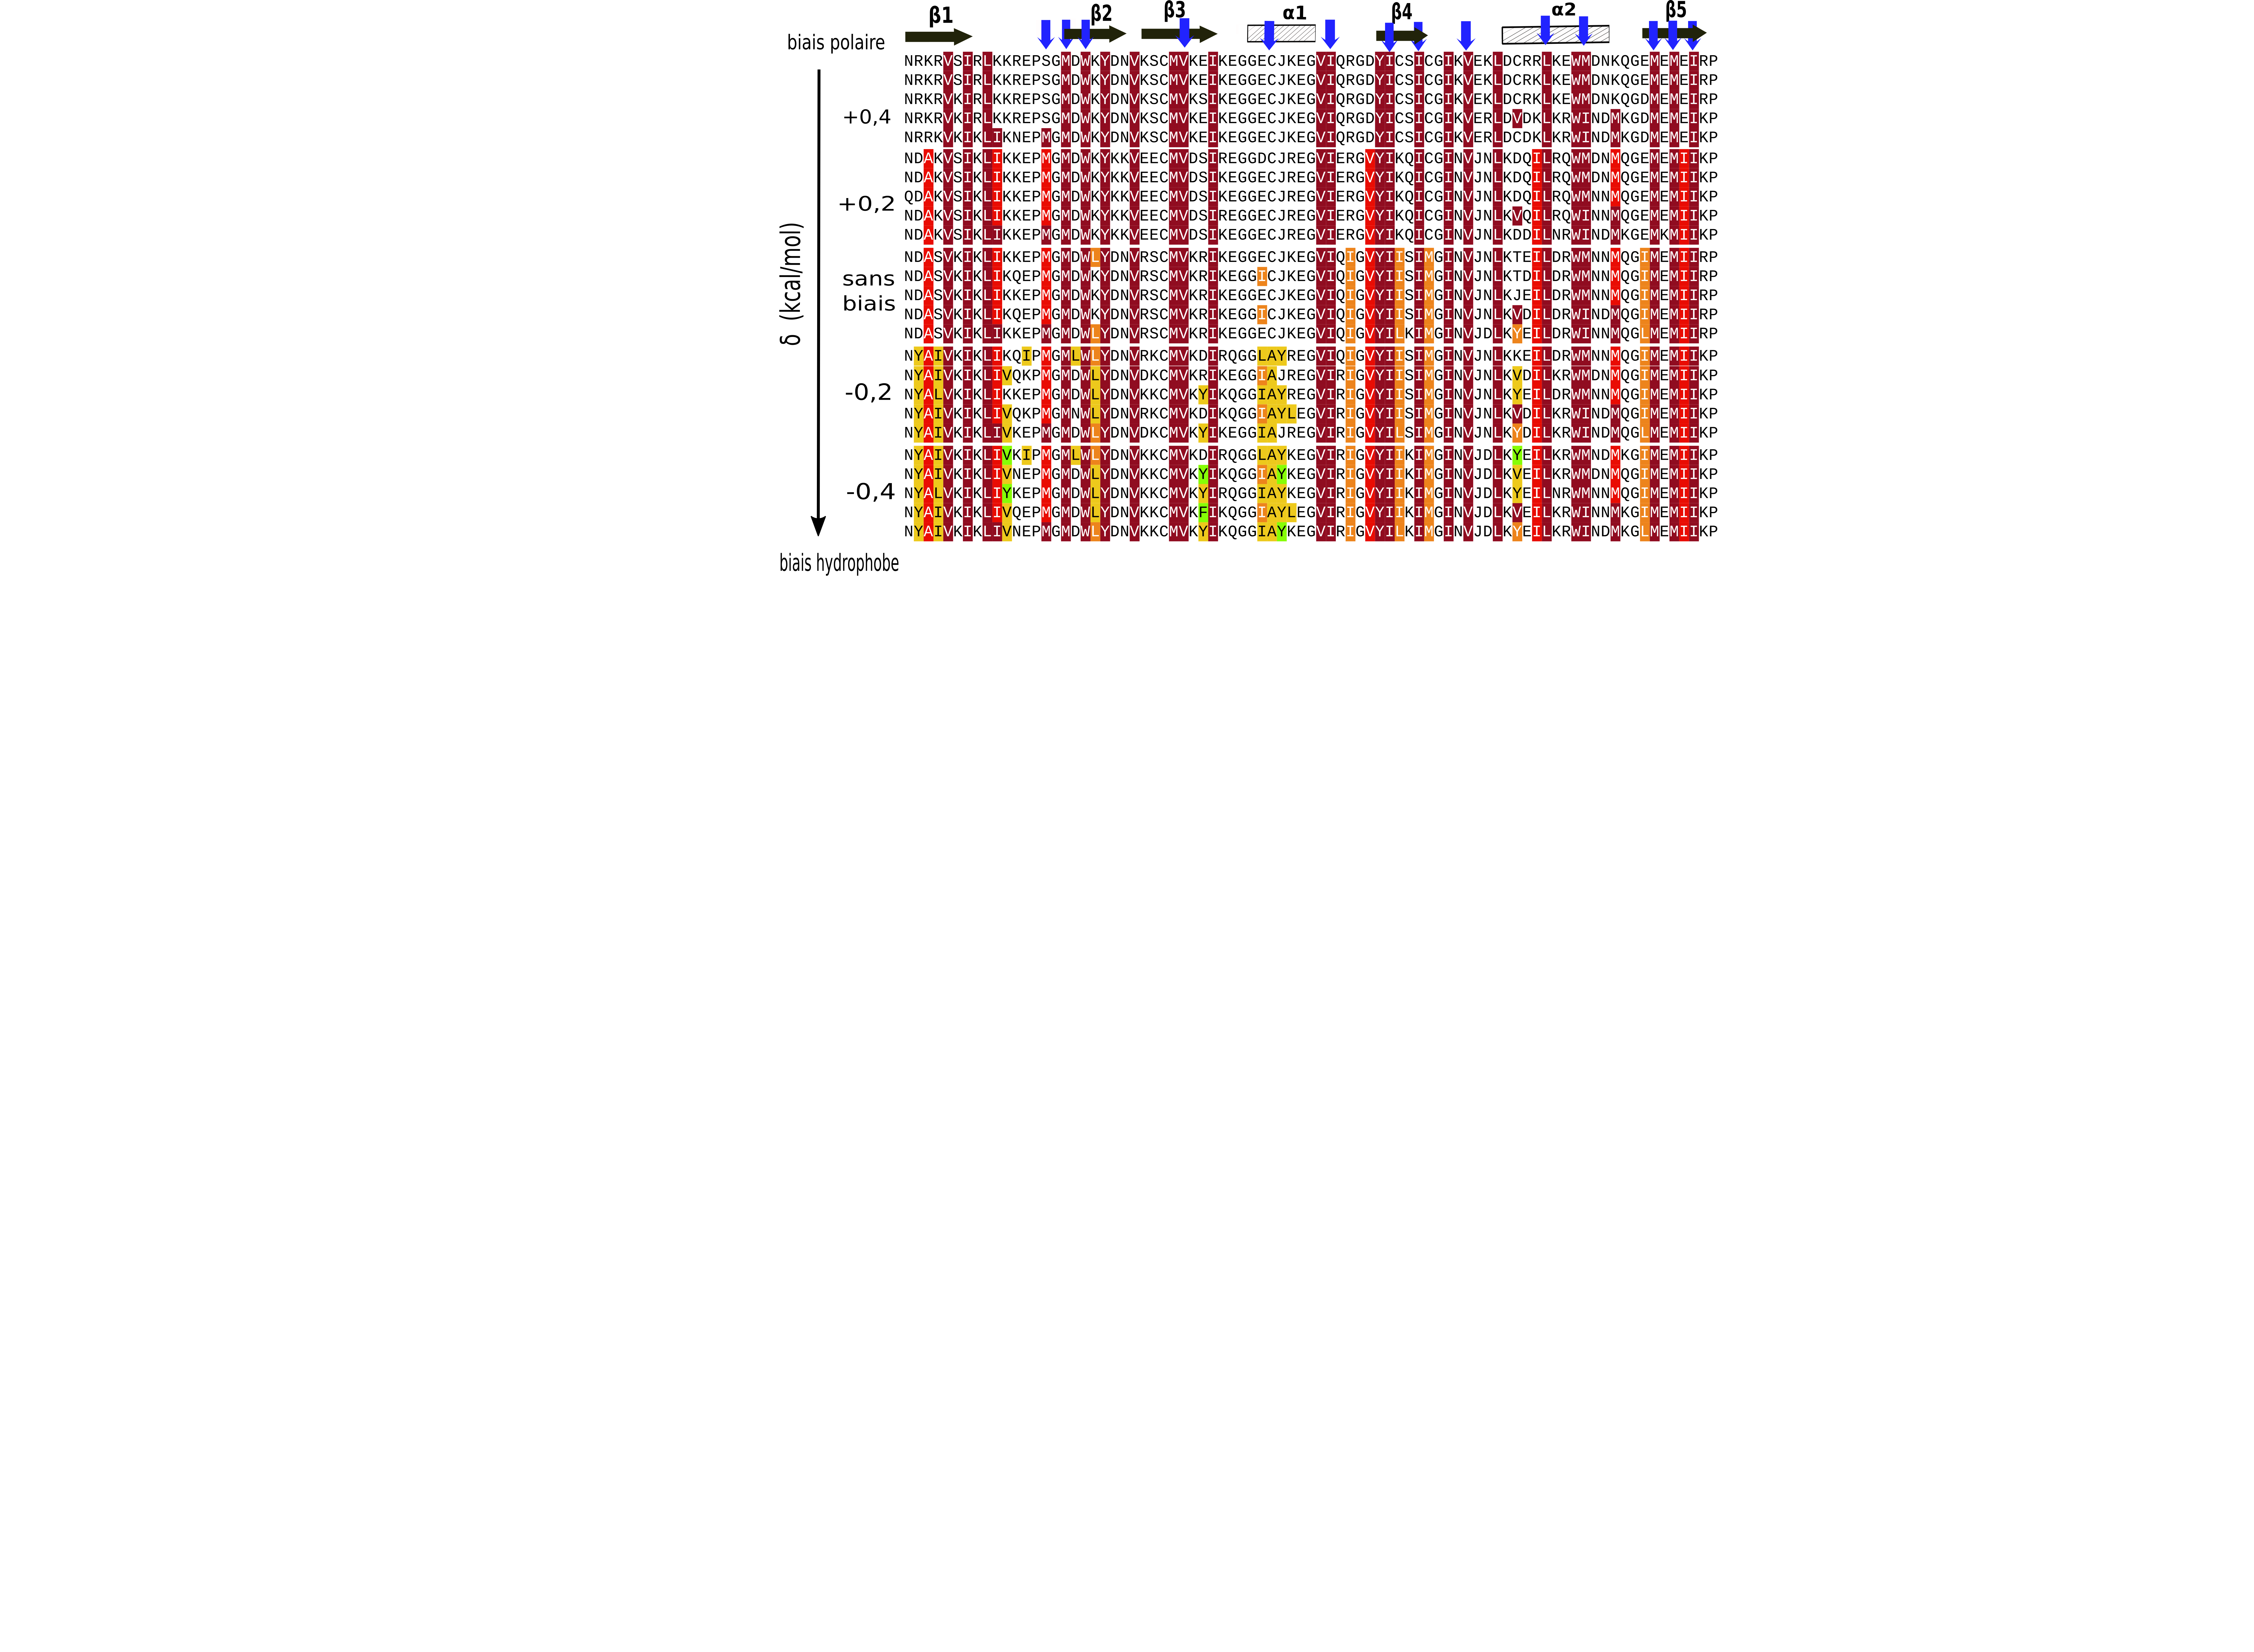
\includegraphics[width=25cm]{titration/alignCASK.png} \\
  \end{tabular}
  
  \caption{\small Séquences Cask obtenues avec un delta des énergies de références à -0,4,-0,2,0,0.2 et 0,4 et la structure native.Les hydrophobes pour des deltas de -0,4,-0,2,0,0.2 et 0,4 sont représentés par un jeu de couleurs allant du rouge foncé au vert clair, en passant par le jaune.}
  \label{titrationAlignCask}
\end{figure}


\includepdf[pages=-]{publicationPDZ.pdf}


\section{Conclusion}

\subsection{modèle mis en œuvre}

Nous avons paramétré notre modèle CPD pour la conception informatique de domaine PDZ, mis en œuvre dans le logiciel Proteus. Pour la modélisation de l'état replié, nous avons utilisé un champ de force protéique de qualité. Nous avons effectué des premiers paramétrages sur un ensemble de 8 domaines PDZ, dont 2 pour évaluer la transférabilité des résultats, avec une première méthode de solvant \og GB \fg, le modèle NEA et une constante diélectrique $\epsilon_P$  égale à $8$. Puis nous avons effectué de nouveaux paramétrages sur un ensemble de 3 domaines PDZ, avec une constante diélectrique $\epsilon_P$  égale à $4$ et avec deux modèles de solvant, le NEA et un second modèle \og GB \fg , le modèle FDB et un jeu de paramètres surfaciques spécifiques. Pour les chaînes latérales, nous utilisons une bibliothèque de rotamères simple et discrète et une petite minimisation de chaque paire pendant le calcul de la matrice d'énergie pour atténuer l'approximation de la discrétisation des rotamères. La fonction d'énergie et la description des rotamères ont été testées de manière approfondie et ont démontré de très bonnes performances pour les tests de reconstruction de chaînes latérales \cite{Gaillard16} (comparable au programme très populaire Scwrl4 (\cite{Krivov09}) ).

La représentation de l'état déplié utilise un modèle simple caractérisé par un ensemble de potentiels chimiques d'acide aminé empiriques ou énergies de référence. Ces énergies sont déterminées par une procédure de maximisation de vraisemblance, décrite ici, afin de reproduire la composition d'acides aminés d'homologues naturels soigneusement sélectionnés. L'état déplié utilisé ici bénécifie d'un raffinement supplémentaire, puisque des valeurs d'énergies de référence distinctes sont utilisées pour les positions d'acides aminés qui soient enfuis soient exposés à l'état replié.  

Cette méthode suppose qu'il existe une structure résiduelle à l'état déplié, où certaines positions sont plus enfuies que d'autres. En outre, cela doit rendre le paramétrage plus robuste et moins sensible à la taille et à la structure des homologues naturels utilisés pour définir les compositions d'acide aminé cibles, car les fréquences d'acide aminé des positions exposées et des régions enfouies sont calculées séparément. En principe, cela double le nombre d'énergie de référence à ajuster. Cependant, nous avons réduit ce nombre en introduisant des classes de similarité d'acide aminé, avec une énergie de référence ajustable par classe. Cette contrainte est levée dans la seconde moitié des cycles d'optimisation. Lors de l'optimisation des énergies de référence, nous effectuons, des calculs de séquences pour chaque protéine de notre jeu de test où une position sur deux peut muter ( à l'exception de Gly et Pro), avec une simulation distincte pour chaque moitié. Ceci de tel sorte que, lors de l'optimisation des paramètres, une position mutable est toujours entourée d'un environnement identique au type sauvage au moins sur les deux positions immédiatement voisines sur le squelette. Les calculs de conception des séquences s'appuient sur une méthode d'exploration Monte-Carlo avec échange de réplique, qui utilise un demi-milliard de pas par simulation et produit des milliers de séquences par simulation.

Le modèle présente plusieurs limitations, dont la plupart se trouvent dans les implémentations et les applications du CPD. La première est l'utilisation de la stabilité des protéines comme seul critère de conception, sans prendre en compte explicitement la spécificité du pli \cite{Schmidt08,Simonson13}, la protection contre l'agrégation , ou des considérations fonctionnelles comme la liaison des ligands. Toutefois, nous notons que les tests superfamily n'ont pas entraînés de mauvaises affectations ( séquences perçues comme préférant un autre pli SCOP), donc en pratique, la spécification du pli est réalisée. Une limitation supplémentaire est introduite  par l'utilisation d'un squelette protéique fixe lors du calcul de la matrice d'énergie. En fait, le squelette n'est pas vraiment fixe. Certains mouvements sont autorisés, mais modélisés implicitement, à travers l'utilisation d'une constante diélectrique protéique supérieure à $1$ ($\epsilon_p= 4$ ou $8$) (\cite{Simonson13}). Cette valeur diélectrique signifie que la structure protéique (y compris son squelette) est autorisée à se détendre ou à se réorganiser en réponse à une redistribution de charge associée à des mutations ou a un changement de rotamères de la chaîne latérale. Cependant, la réorganisation est modélisée non pas explicitement, mais implicitement (\cite{Simonson13}), et elle n'implique pas de mouvement des centres atomiques ou de leur sphère de Van der Waals associée. Ainsi, le squelette ne peut ni se réorganiser en réponse à une répulsion stérique produite par des mutations ou des changements de rotamères ni se déplacer pour remplir l'espace laissé vide par une mutation.  
L'utilisation d'un squelette fixe peut être en partie compensée en concevant plusieurs structures PDZ. Par exemple, la mise en commun des séquences calculées sur 6 protéines a donnée une entropie moyenne de séquence nettement plus proche de cette de l'ensemble expérimental  Pfam. Une nouvelle méthode pour la conception de protéine multi-backbone a récemment été développée dans Proteus, sur la base d'une méthode Monte-Carlo hybride qui préserve l'échantillonnage de la distribution de Boltzmann \cite{Druart17}. Cette méthode pourra être appliquée dans les prochaines études.
Une autre limitation de notre modèle est la nécessité, pour des résultats optimaux, de paramètres les énergies de référence spécifiquement pour un ensemble donné de protéines. Cette étape est bien automatisée et de façon très parallèle. Cependant, cela implique plusieurs choix qui sont partiellement arbitraires. Ceux-ci comprennent le choix d'un ensemble de domaines protéiques pour représenter la protéine ou la famille d'intérêt. Nous devons également choisir un seuil de similarité pour définir les homologues cibles à partir desquels sont calculées les compositions expérimentales d'acides aminés. Ici, nous avons choisi d'utiliser les homologues de chaque membre de la famille, de calculer leurs compositions, puis la moyenne sur l'ensemble des familles. Cette méthode a correctement fonctionné, mais d'autres choix sont possibles et des travaux complémentaires sont nécessaires pour pouvoir tirer des conclusions définitives sur ces choix.

Une autre limitation est l'utilisation d'un modèle de solvatation dans lequel l'environnement diélectrique de chaque paire de résidus est supposé ici être celui de la structure native (ce qu'on appelle \og Approvisionnement environnemental natif\fg ou NEA \cite{74},\cite{76}). Cela permet d'avoir une fonction énergétique décomposable sur les paires de résidus et peut être précalculée et stockée. Certaines de ces limitations sont supprimées dans le modèle FDB. En particulier, comme la fonction d'énergie est principalement basée sur la physique, elle a pu être améliorée par implémentations d'un calcul GB plus exact. Par ailleurs, il a été mis en place un modèle amélioré pour la solvatation hydrophobe, qui est plus rapide et plus précise que notre terme d'énergie de surface actuelle (article en préparation).

\subsection{tests et application}

Les séquences conçues par Proteus sont comparées aux séquences naturelles, à travers des tests de reconnaissance du pli, des calculs de similarité, des calculs d'entropie et des taux d'identité de séquences. Dans les simulations, nous concevons la totalité de la séquence de la protéine, de sorte que toutes les positions  ( à l'exception de Gly et Pro) peuvent muter librement, soumis à la seulement contrainte de générer une composition moyenne en acides aminés similaire à la composition moyenne expérimentale ( à travers les énergies de références). Malgré la quasi absence de contrainte expérimentale, les séquences obtenues ont une forte similitude globale avec les séquences naturelles de Pfam, mesurée par les scores de similarité Blosum40. Les scores obtenus sont, pour l'essentiel, comparables aux scores de similarité entre les paires de séquences Pfam entre elles. La similitude est très forte pour les résidus au cœur de la protéine, comme cela a été observé dans des études CPD précédentes (\cite{30},\cite{72}). En revanche, pour les résidus pris sur l'ensemble de la protéine, les scores de similarité sont plus faibles, mais l'approximation FDB couplée à une constante diélectrique $\epsilon_p$ égale à 4 donne toujours des séquences similaires à des homologues naturels modérément éloignés.

Notez que de nombreux résidus de surface sont impliqués dans des interactions fonctionnelles, comme les onze résidus de liaison aux peptides dans les domaines PDZ. Les résidus de surface sont également sélectionnés selon l'évolution pour éviter l'agrégation ou des adhésions indésirables. Ces contraintes fonctionnelles ne sont pas explicitement prises en compte dans notre protocole de design.  Malgré ces difficultés sur les résidus de surface, la reconnaissance de pli avec l'outil Superfamily  appliquée aux meilleurs modèles conçus est presque parfaite. Les tests de reconnaissance de plis antérieurs qui utilisaient une fonction d'énergie plus simple donnaient un taux de reconnaissance de pli inférieur, à environ 85\% (pour un ensemble de tests plus large et plus diversifié) et des similitudes inférieures (\cite{15},\cite{50}).De toute évidence, l'utilisation combinée d'un champ de force protéique amélioré, du solvant GB FDB et des énergies de référence spécifiques à la famille conduisent à des séquences calculées proches des séquences natives.
Les séquences Proteus ont également été comparées aux séquences obtenues avec le logiciel Rosetta , qui a lui-même été testé de manière approfondie. Sur la Base des scores de similarité de Blosum (par rapport aux séquences naturelles dans Pfam) et des tests de reconnaissance du pli, les séquences Proteus et Rosetta sont globalement de même qualité. Cependant, Rosetta fait moins de mutations que Proteus; de sorte que les scores d'identité, par rapport à la protéine de type sauvage correspondante, sont entre 7\% et 9\% plus haut chez Rosetta que pour la version FDB de notre modèle. Ce qui veut dire que Proteus modifie environ 5 positions en plus, en moyenne, par domaine PDZ. 



   

%%% Local Variables:
%%% mode: latex
%%% TeX-master: "../these"
%%% End:
